% VLDB template version of 2020-08-03 enhances the ACM template, version 1.7.0:
% https://www.acm.org/publications/proceedings-template
% The ACM Latex guide provides further information about the ACM template

\documentclass[sigconf, nonacm]{acmart}

%% The following content must be adapted for the final version
% paper-specific
\newcommand\vldbdoi{XX.XX/XXX.XX}
\newcommand\vldbpages{XXX-XXX}
% issue-specific
\newcommand\vldbvolume{14}
\newcommand\vldbissue{1}
\newcommand\vldbyear{2020}
% should be fine as it is
\newcommand\vldbauthors{\authors}
\newcommand\vldbtitle{\shorttitle} 
% leave empty if no availability url should be set
\newcommand\vldbavailabilityurl{URL_TO_YOUR_ARTIFACTS}
% whether page numbers should be shown or not, use 'plain' for review versions, 'empty' for camera ready
\newcommand\vldbpagestyle{plain} 
\usepackage{pifont}
\usepackage{url}
\usepackage{subfigure}
\usepackage[ruled]{algorithm2e}
\usepackage{algorithmic}
\usepackage{bbding}
\begin{document}
\title{GSnap: An Efficient Group-based Snapshot Index in the Cloud Database}

%%
%% The "author" command and its associated commands are used to define the authors and their affiliations.

\author{Xiaoshuang Peng$^1$, Xiaopeng Fan$^1$, Chuliang Weng$^1$$^\ast$, Shi Cheng$^2$, Lingbin Meng$^2$, Cuiyun Fu$^2$, and Feifei Li$^2$}
\affiliation{%
	  \institution{
	     East China Normal University$^1$,
	  Alibaba Group$^2$
						}
	}

%\email{{xspeng, xpfan}@stu.ecnu.edu.cn, clweng@dase.ecnu.edu.cn, 
%	{chengshi.cs, lingbin.mlb, cuiyun.fcy, lifeifei}alibaba-inc.com}
\email{{xspeng, xpfan}@stu.ecnu.edu.cn, clweng@dase.ecnu.edu.cn,}

\email{{chengshi.cs, lingbin.mlb, cuiyun.fcy, lifeifei}@alibaba-inc.com}

%\author{J\"org von \"Arbach}
%\affiliation{%
%  \institution{University of T\"ubingen}
%  \city{T\"ubingen}
%  \country{Germany}
%}
%\email{jaerbach@uni-tuebingen.edu}
%\email{myprivate@email.com}
%\email{second@affiliation.mail}
%
%\author{Wang Xiu Ying}
%\author{Zhe Zuo}
%\affiliation{%
%  \institution{East China Normal University}
%  \city{Shanghai}
%  \country{China}
%}
%\email{firstname.lastname@ecnu.edu.cn}
%
%\author{Donald Fauntleroy Duck}
%\affiliation{%
%  \institution{Scientific Writing Academy}
%  \city{Duckburg}
%  \country{Calisota}
%}
%\affiliation{%
%  \institution{Donald's Second Affiliation}
%  \city{City}
%  \country{country}
%}
%\email{donald@swa.edu}

%%
%% The abstract is a short summary of the work to be presented in the
%% article.
\begin{abstract}
Many cloud databases provide fine-grained regular snapshots and sparsely deleted snapshots based on importance, and dynamically maintain large-scale snapshots to ensure data security and mine the value of cold data.
However, in the existing snapshot technologies, the write amplification feature of Copy-on-Write (CoW) introduces additional expensive I/O operations in the cloud environment. In the Redirect-on-Write (RoW), the modified data blocks are scattered among the snapshots, resulting in a dependency between the snapshots, which seriously affects the recovery performance.

In this paper, we observed that the access of snapshots has the characteristics of locality and continuity. We therefore propose an efficient RoW-based snapshot mechanism, called GSnap, which groups snapshot indexes according to cloud database workload and access behavior of snapshot. Specifically, we use two key techniques: Shared-Subtrees Indexing (SSI) and Group-Based Dividing (GBD), to perform split dependency of snapshot index.
In-group snapshot indexes reduce memory overhead by sharing subtrees. The snapshot index dependency chain is divided into groups and there is no dependency on snapshot indexes between groups.
The index can directly locate data blocks instead of iterative traversal.
At the same time, the design of the snapshot index deletion method is adapted to the snapshot sparse deletion model.
We have implemented a prototype system in Ceph. 
Evaluation results with datasets demonstrate that, compared with state-of-the-art techniques, GSnap could effectively balance the overhead between index memory usage and recovery time.
\end{abstract}

\maketitle

%%% do not modify the following VLDB block %%
%%% VLDB block start %%%
%\pagestyle{\vldbpagestyle}
%\begingroup\small\noindent\raggedright\textbf{PVLDB Reference Format:}\\
%\vldbauthors. \vldbtitle. PVLDB, \vldbvolume(\vldbissue): \vldbpages, \vldbyear.\\
%\href{https://doi.org/\vldbdoi}{doi:\vldbdoi}
%\endgroup
%\begingroup
%\renewcommand\thefootnote{}\footnote{\noindent
%This work is licensed under the Creative Commons BY-NC-ND 4.0 International License. Visit \url{https://creativecommons.org/licenses/by-nc-nd/4.0/} to view a copy of this license. For any use beyond those covered by this license, obtain permission by emailing \href{mailto:info@vldb.org}{info@vldb.org}. Copyright is held by the owner/author(s). Publication rights licensed to the VLDB Endowment. \\
%\raggedright Proceedings of the VLDB Endowment, Vol. \vldbvolume, No. \vldbissue\ %
%ISSN 2150-8097. \\
%\href{https://doi.org/\vldbdoi}{doi:\vldbdoi} \\
%}\addtocounter{footnote}{-1}\endgroup
%%%% VLDB block end %%%
%
%%%% do not modify the following VLDB block %%
%%%% VLDB block start %%%
%\ifdefempty{\vldbavailabilityurl}{}{
%\vspace{.3cm}
%\begingroup\small\noindent\raggedright\textbf{PVLDB Artifact Availability:}\\
%The source code, data, and/or other artifacts have been made available at \url{\vldbavailabilityurl}.
%\endgroup
%}
%%% VLDB block end %%%

\section{Introduction}
Cloud Block Storage (CBS) is an important data storage technique in cloud computing, such as Amazon Elastic Block Store (EBS) \cite{varia2014overview}, Openstack Cinder \cite{shrivastwa2016openstack}, Sheepdog \cite{morita2010sheepdog} and Ceph RBD \cite{weil2006ceph,weil2007rados}. CBS usually partitions storage devices into logical data blocks and treats them as objects that are ultimately stored in the storage cluster. Its advantage is to decouple the upper different storage interfaces from the lower storage devices. But the accessing overhead cannot be ignored because of the additional computational and network overhead in the cloud environment.

Though CBS provides reliability and persistence, tenants still keep taking snapshots continuously, to store the state of the block device at various times for auditing, separating heavy business, and spatial data mining. In particular, the snapshot only stores data blocks that have been modified during the process of taking the snapshot, which could greatly decrease storage overhead. However, existing snapshot technologies have some open issues. For Copy-on-Write (CoW) \cite{nightingale2008rethink,chidambaram2013optimistic}, it introduces write amplification because new data writed to the data block are kept in place. But the old data block, which is now part of the snapshot, is explicitly copied to a new location. For Redirect-on-Write (RoW), the updated data blocks are scattered in the snapshots instead of the block device. So restoring a snapshot may access multiple snapshots, resulting in significant additional cost in the cloud.

The user could access the database replicate once mounting a snapshot of the block device, and typically access the snapshot set for the applications \cite{yang2011st,joseph2019securing,pekerskaya2006mining}, which is also verified by the snapshot set query of AliCloud \cite{alibackupset}. The tenant typically takes snapshots of the database periodically and loads the snapshot collection over time. The length of the snapshot set is determined by the query date. Besides, they may combine multiple snapshot sets for cross-querying.
In terms of RoW, many works tend to build data block indexes \cite{tsikoudis2020rid,tsikoudis2018rql,shrira2005snap} to accelerate the restoration process. They cache the mapping from data block numbers to physical block addresses, which helps achieve a higher access data block speed. However, fragmentation inevitably becomes worse with high generation snapshots, restoring the snapshot requires loading all the reference snapshots' indexes, which takes time. Amazon EBS snapshot \cite{AmazonEBSSnapshot} keeps all regions' (continuous unaltered data block area) positions to prevent snapshot dependency, but the space overhead for each snapshot cannot be overlooked.

Based on the workload of the database and the snapshot access characters, we propose a simple but effective snapshot index structure based on RoW, which balances the overhead of recovery time and index memory consumption. The snapshot dependence chain is divided into groups, with each snapshot index relying son the previous snapshots in its group but not on snapshots outside the group. 
By sharing the subtrees when taking snapshots in a group, the data block address could be obtained directly and then the index memory overhead is decreased. Besides, prefetching snapshots in a group instead of dependent snapshots when restoring a version, which could significantly reduce the number of snapshots and the recovery time. But grouping snapshot seems to be a non-trivial challenge. First, how to cut off the dependency between snapshots and share subtrees in a group? Second, how to adjust the length of a group to adapt to the users' access and update frequency?

We present the group-based snapshot index, called GSnap, to solve the issues above. GSnap has two key technologies, there are Shared-Subtrees Indexing (SSI) and
Group-Based Dividing (GBD). SSI sets two types of indexes in a group. Specifically, The first snapshot index is the complete B+ tree, and the subsequent snapshots are partial. The complete tree no longer depends on the former indexes, while the partial tree nodes point to those previous indexes in the group, effectively reducing redundancy.
GBD divides the group according to the snapshot update ratio and the recent average continuous access length. 
The purpose is to load only one snapshot group when the snapshot is recovered.

Subsequently, we implement GSnap, with SSI and GBD technologies.
GSnap can balance the time and space overhead in snapshot recovery, while we adjust the GSnap deletion according to the sparse snapshot deletion mechanism.
We integrated GSnap index into Ceph RBD that supports taking snapshots at scale and recovering from any snapshot with low latency. We employ workloads derived from the standard TPC-C benchmark to evaluate the performance snapshot index GSnap . 


To sum up, we make the following contributions:
\begin{itemize}
	\item We propose GSnap, a high-performance snapshot index that could directly locate data blocks and balance the overhead of recovery time and index memory consumption.
	\item We design a group-based snapshot deletion method to adapt to the sparse snapshot deletion mechanism, which could effectively speed up snapshot deletion.
	\item We implement GSnap based on Ceph RBD. Evaluation shows that GSnap gains significant performance improvement against state-of-the-art block storage systems.
\end{itemize}

The rest of this paper is organized as follows. Section \ref{Background} presents background. The motivation is introduced in Section \ref{Motivation}. The design and implementation of GSnap are proposed in Section \ref{Design}. The performance evaluation is shown in Section \ref{Evaluation}. Section \ref{Relatedwork} discusses the related work and Section \ref{Conclusions} concludes the paper.

\section{Background}
\label{Background}

\subsection{Cloud Block Storage}
More and more tenants deploy applications and store data on the cloud now.
Cloud Block Storage (CBS) \cite{zhou2018lea,jin2019reasoning,zhang2020osca} could provide large-volume storage devices for Elastic Compute Service. As shown in Figure \ref{fig:CBS}, CBS is made up of the client layer, data forwarding layer, and storage server layer. 
The client layer presents tenants with the view of elastic and isolated logic block devices allocated according to the configuration and mounted to the client virtual machines. The block device is usually divided and striped into objects of the same size for storage and the object size can be configured in the storage server.
The data forwarding layer maps data block physical location from the object number, and forwards I/O requests from the client to the storage server through a two-level hashing \cite{karger1997consistent,weil2006crush}, which spread replicas of an object to different nodes. Similarly, Openstack Swift \cite{ring} stores objects in partitions and transfer replicas of partitions to different regions by the ring, which is used to record the location information. 
The storage cluster layer is responsible for providing physical storage and typically employs replications to ensure data reliability and availability. Therefore, compared with the local block devices, the requests of CBS to access the data block inevitably pass through three layers to the storage cluster, and incur the overhead of additional address calculation and network transmission.

\begin{figure}[t]
	\centering
	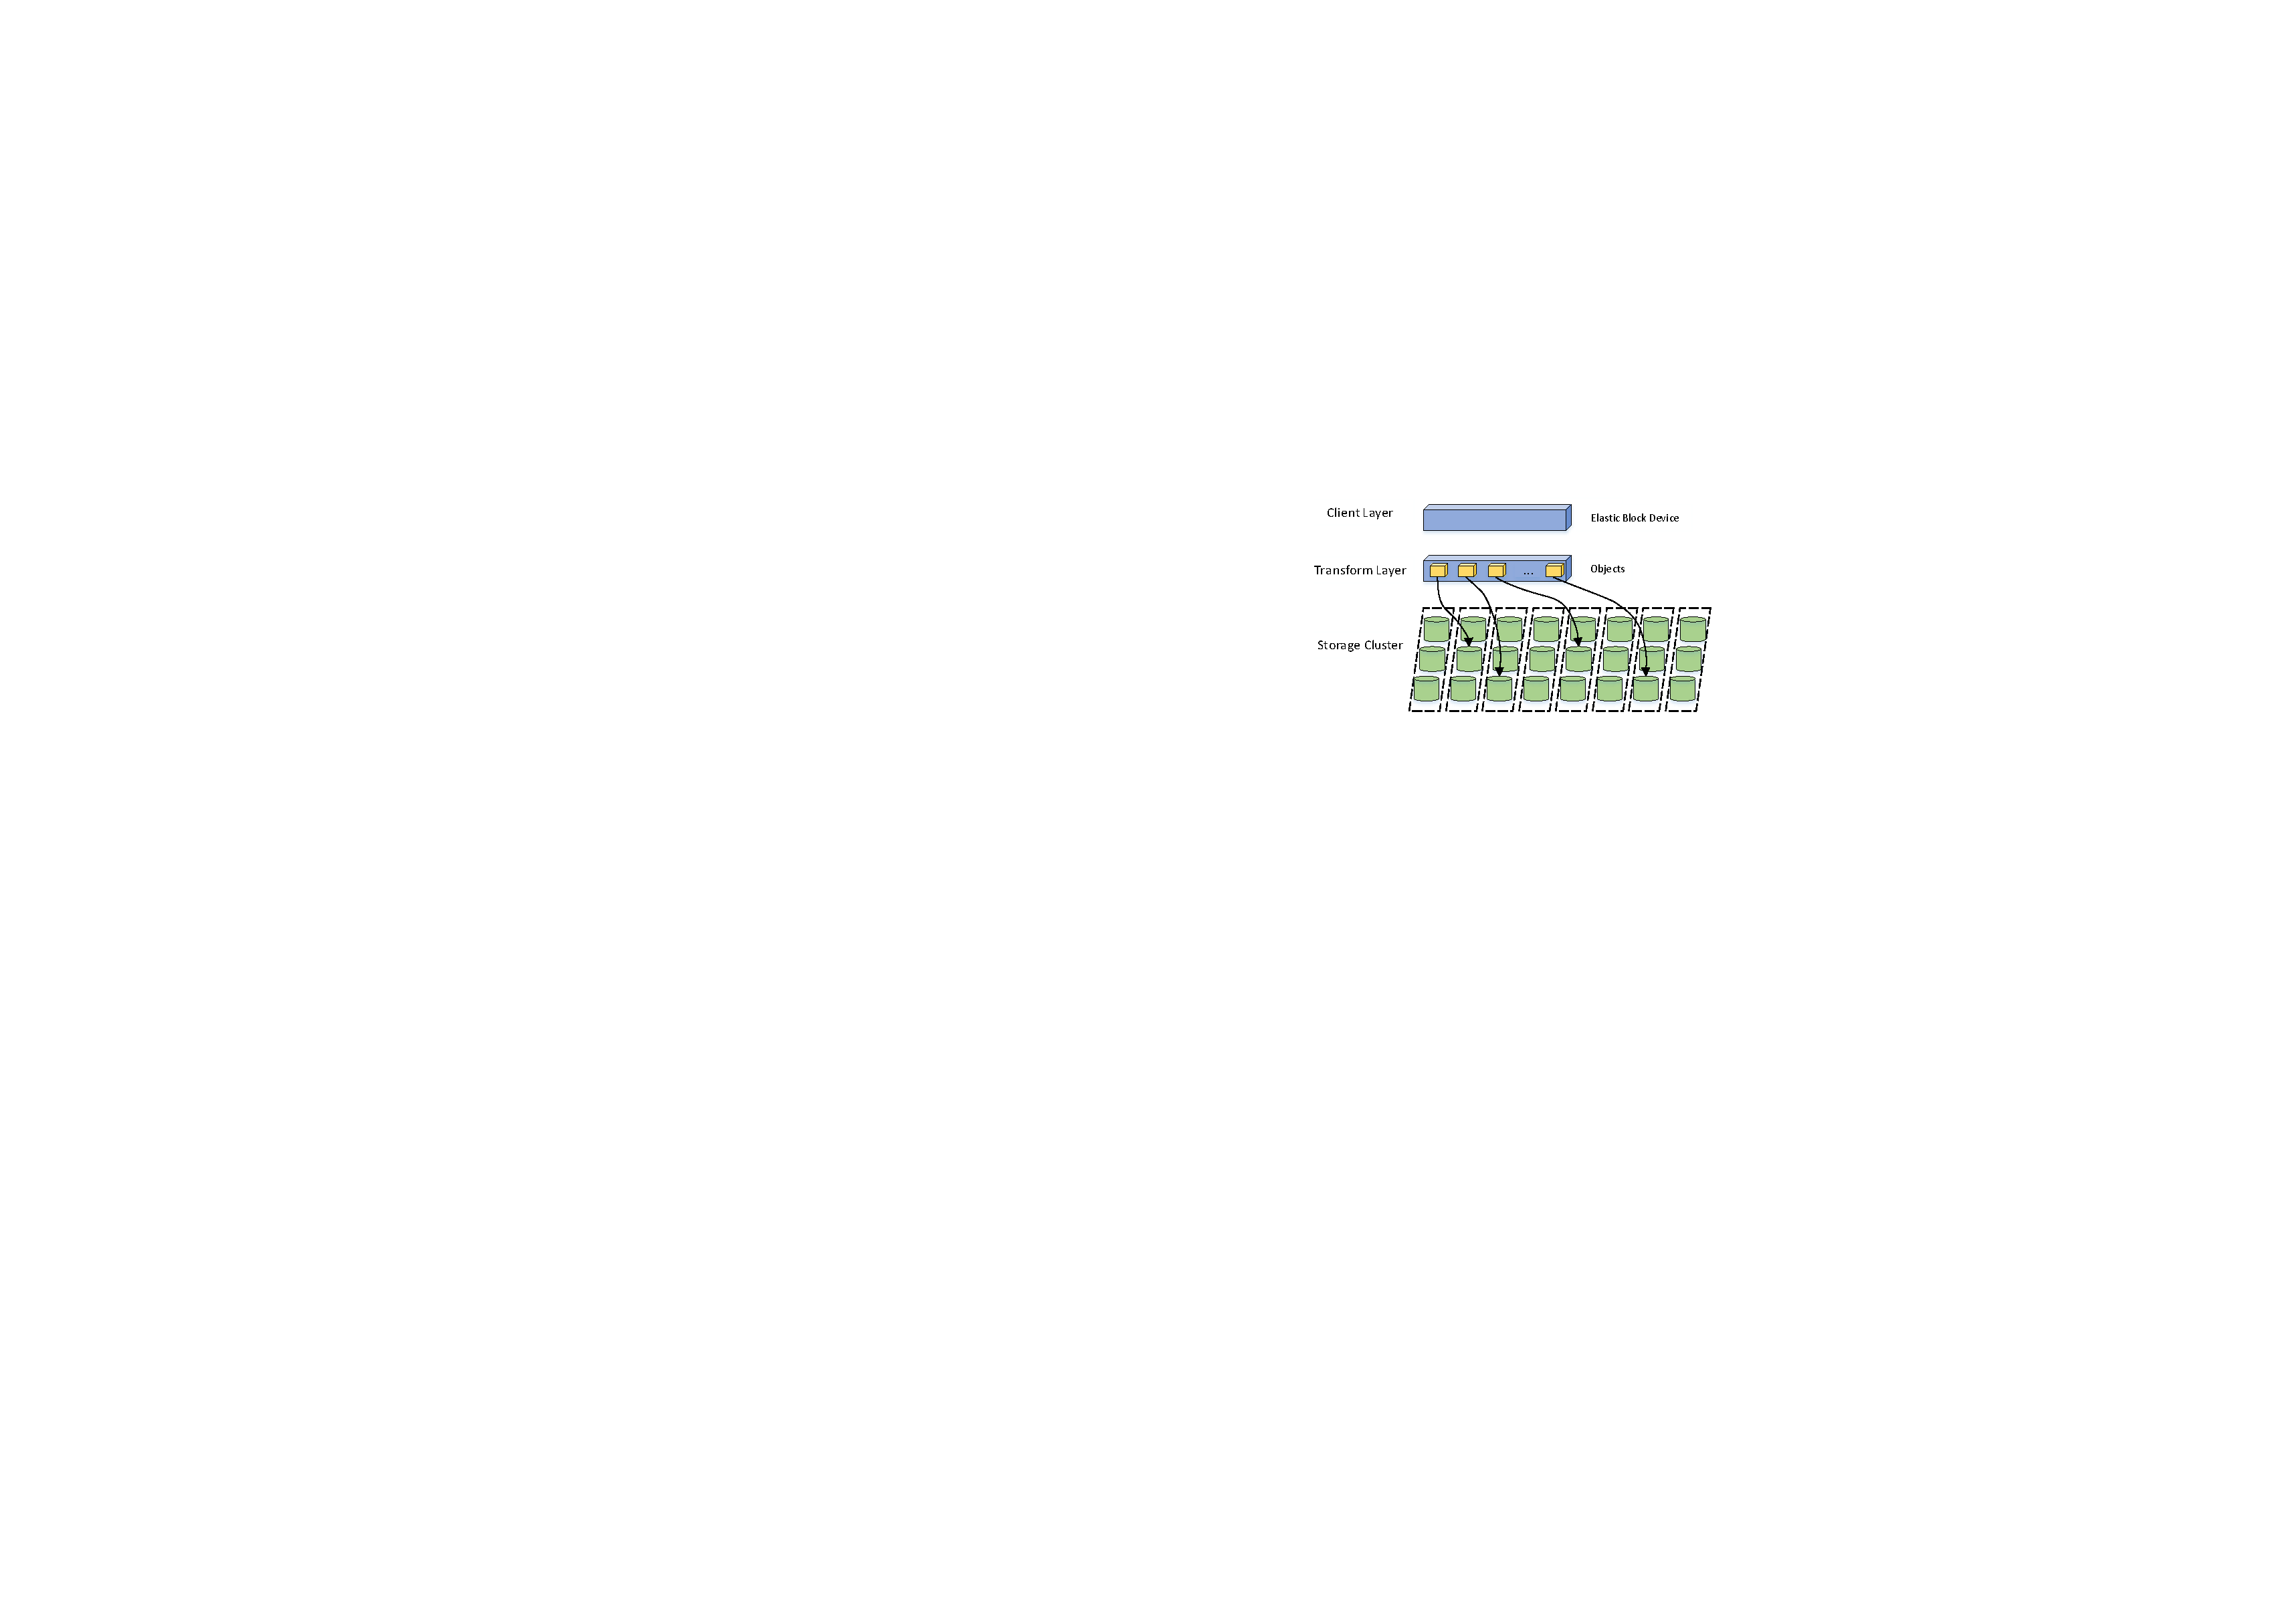
\includegraphics[width=8cm]{figures/ceph_pic/blockdevice.pdf}
	\caption{Architecture of Cloud Block Storage}
	\label{fig:CBS}
\end{figure}

\subsection{Snapshot Implementations}
There are many classic snapshot technologies, such as CoW, CoW with background copy (CoW+), Split Mirror Redundant Array of Independent Disks (SMRAID), Incremental Snapshot, Continuous Data Protection (CDP) \cite{garimella2006understanding}, and RoW. The different types of snapshot technologies have been extensively compared and analyzed \cite{mahipal2021virtual,joseph2019securing,almulla2013distributed,subramanian2014snapshots}. In summary, the write overhead of CoW, CoW+, and SMRAID are suffered by their methodologies, their derivative technologies induce overheads for regular I/O and dramatic increase of sync operations when snapshots are present \cite{subramanian2014snapshots,li2012irow}. Incremental Snapshot and CDP are mostly dependent on the underlying technology used for taking snapshots and network bandwidth.

For RoW-based snapshots, new data blocks write to the blocks belonging to the current snapshot, which stores the previous version number for all old data blocks.
RoW sacrifices contiguity in the original copy for lower overhead updates in the presence of snapshots. 
As the system runs and takes snapshots over a long time, the fragmentation of the data block becomes increasingly serious. When locating the data block, the snapshot checks whether it exists in the snapshot. If not, the snapshot continues to look for the earlier snapshots.
Iterative search degrades performance due to the low update frequency of data blocks and the massive amount of snapshots.
Amazon EBS \cite{varia2014overview} has an optimized RoW snapshot index that stores the regions, which are continuous unchanged data blocks. The region points to the last changed snapshot instead of the previous snapshot to avoid iterative queries.
However, when the number of snapshots grows, the size of each region shrinks and the number of regions grows, considerably increasing the memory footprint of indexes.

\subsection{Vary Layers Supported Snapshot}
\begin{table}[htbp]
	\centering
	\caption{Summary of existing methods for the database backup and recovery (FS: file system, DB: database)}
	\label{table:snapshot_layer}
	\resizebox{\columnwidth}{9mm}{
		\begin{tabular}{|c|c|c|c|c|}
			\hline
			Methods       & Mysqldump & Xtrabackup & BTRFS & LVM   \\ \hline
			layer         & DB        & DB         & FS    & Block \\ \hline
			backup speed  & slow      & slow       & fast  & fast  \\ \hline
			restore speed & slow      & medium     & fast  & fast  \\ \hline
	\end{tabular}}
\end{table}

Snapshot technology can be implemented at different layers. Table \ref{table:snapshot_layer}  shows the existing methods supported by varying layers.

In the database layer, database administrators can choose mysqldump \cite{mysqldump} for logical backup and Percona Xtrabackup \cite{xtrabackup} for physical backup. A logical backup stores the queries executed by transactions, while a physical backup copies the raw data to storage. In the recovery process, the stored queries are re-executed, or backup data are copied to a database directory. However, recovery operations in the existing tools take a long time, since these recovery procedures involve a large amount of I/O operations induced by database queries. Xtrabackup does not perform transactions and only copies original data, and then it is faster than mysqldump in restoring process, but the overhead still cannot be ignored. 

Snapshots techniques supported by file systems and the block layer can be adopted to the backup and recovery of a database. Network Appliance NAS filers, the Sun ZFS filesystem \cite{rodeh2003zfs} and BTRFS \cite{rodeh2013btrfs} organize the file as a tree with data at the leaf level and meta-data maintained in internal nodes. Each snapshot consists of a separate tree, but the snapshot may share subtrees with other snapshots. When the user produces a snapshot of the volume, simply duplicates the root node of the original volume as the new tree root node of the snapshot, and the new tree root is pointed to the same children as the original volume.  
Though creating a snapshot is light, the overhead of first write to a block is heavy because the entire tree of meta-data nodes needs to be copied and linked to the root node of the snapshot. 
LVM \cite{hasenstein2001logical} operates between the file system and the storage device and provides fast snapshot creation and restoration using CoW. However, the CoW approach negatively affects run-time performance since it performs redundant writes due to data copies.
We adopt tree structure to organize its data blocks like Parallax \cite{DBLP:conf/eurosys/MeyerACLFHW08} and Ramdisk \cite{nielsen1999use} to support rapid creation of snapshots.

\subsection{Characters of Accessing Snapshots}
\label{Characters}
In this subsection, we present our key observations about the behaviors of accessing snapshots. The characters can be exploited to greatly help design an optimal snapshot index that accelerates snapshot restoring and reduces index memory overhead.

As shown in Figure \ref{fig:retained_distribution}, we collect one-month snapshot information from AliCloud \cite{alibackupset}. There were 115210 snapshots are preserved in the first two weeks, 522086 snapshots in the third week, and 634767 snapshots in the fourth week. Most of the snapshots saved in the last two week, because the system periodically takes snapshots at a fine density and filters snapshots based on the importance and date, which means continuously deleting snapshot sets of different lengths rather than batch deletion. 
Besides, earlier snapshots are easily deleted and merged.
We also count snapshot accessed distribution, as shown in Figure \ref{fig:accessed_distribution}. There are 2091 snapshots accessed within the first day, which accounted for 83.4\% of the snapshots accessed throughout the month. Therefore, the feature of snapshot accessed is temporal locality.

%At the same time, snapshots are mostly recovered in a continuous manner. 

Auditing and fact-checking \cite{jo2019aggchecker,shaull2008skippy} are essential for applications now more than ever. 
In the multiple snapshot scenario, the user may retain the most accessed and recent snapshot set \cite{vrable2009cumulus} to take unanticipated queries on long-term status.
Besides, snapshots are usually loaded in deduplication systems as batches \cite{ren2021accelerating,zou2021dilemma}.
The recovered snapshots are continuous and the length is indeterminate.
Thus, the access behavior of snapshots is continuous. This behavior is proper for cloud tenants, who recover and mount  more snapshots on different machines.

%Finally, we observed that the number of snapshots accessed in the last week is 47$\%$ of the snapshots accessed in a month.
%In a short, users typically access the most recent snapshots continuously.

Existing RoW-based snapshot technologies suffer under continuous snapshot access workloads. The reason is that the dependency between snapshots leads to loading all snapshots with reference relationships into memory instead of only snapshots accessed. The Amazon EBS snapshot index is a complete tree that stores all region's addresses to eliminate the dependency. However, it causes significant pressure on memory consumption because all indexes in memory are complete trees.

%\begin{figure}[t]
%	\centering
%	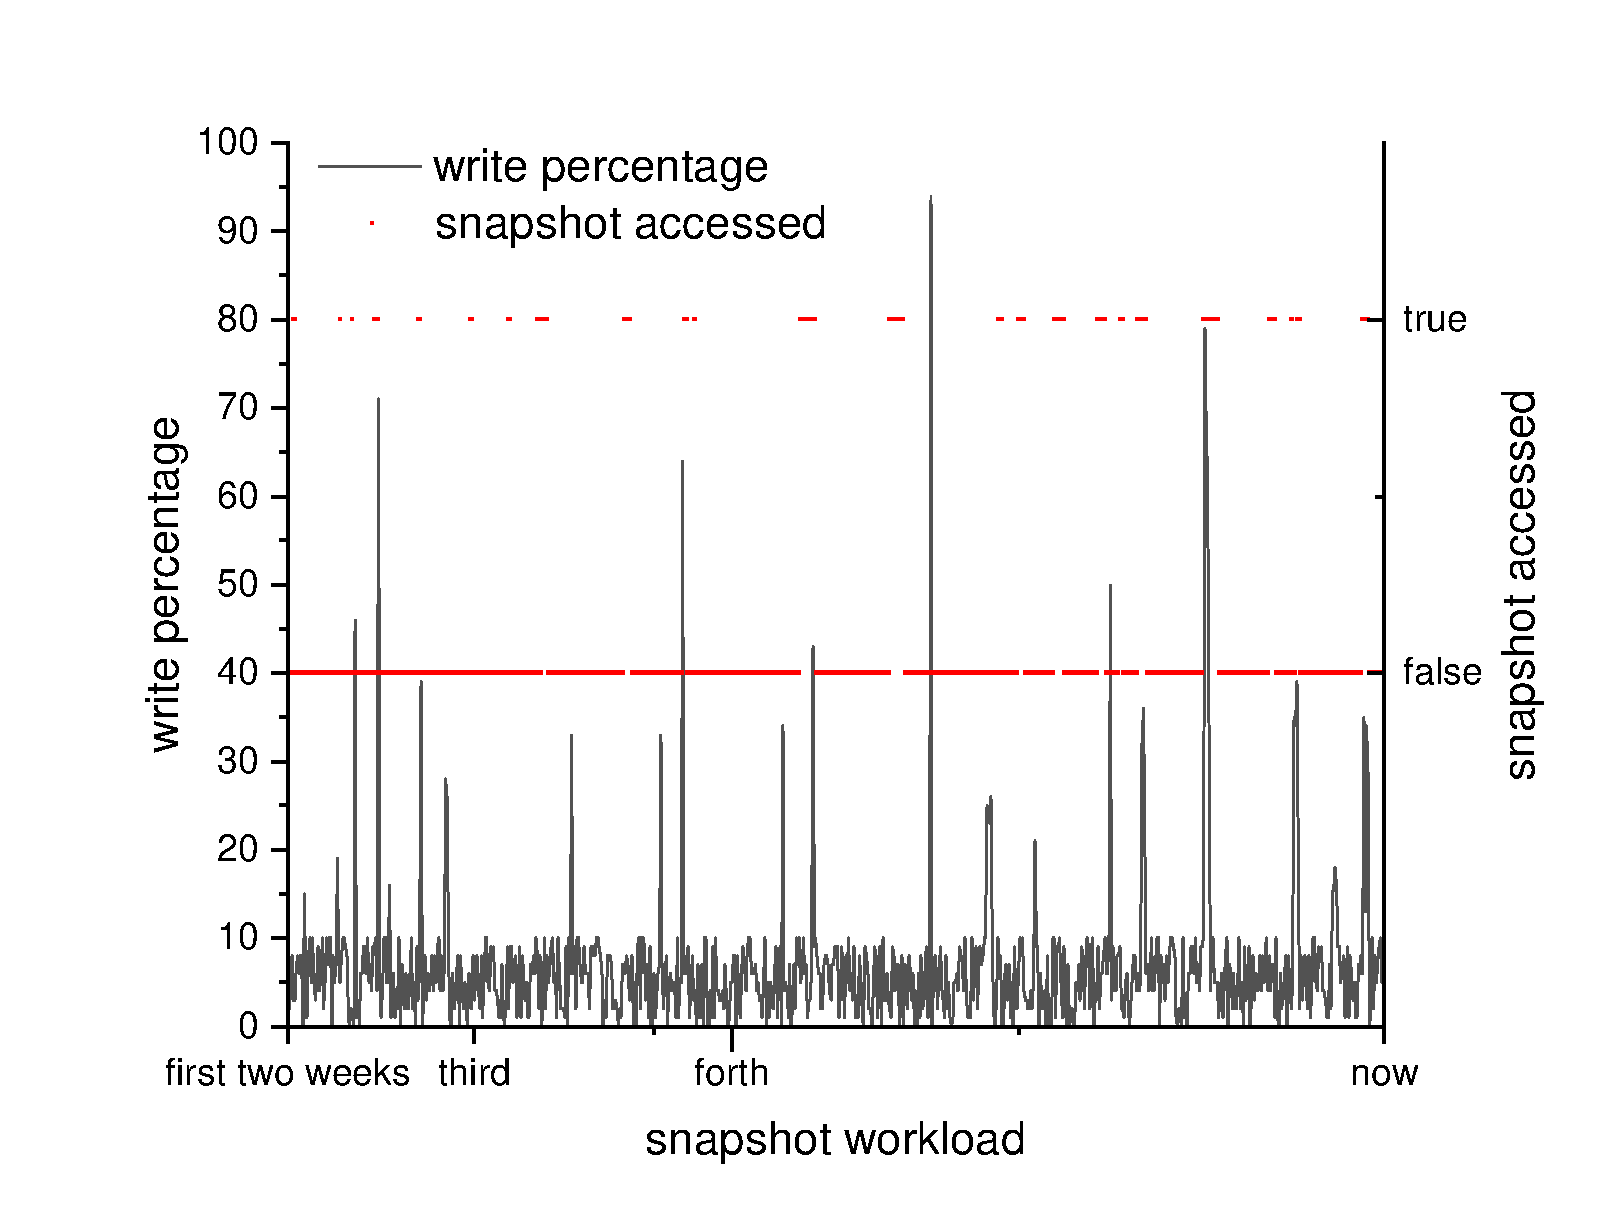
\includegraphics[width=8cm]{figures/ceph_pic/ali_workload.pdf}
%	\caption{Snapshot workload in AliCloud}
%	\label{fig:ali_snapshot_workload}
%\end{figure}
%\vspace{-0.2cm}

\begin{figure}[htbp]
	\begin{minipage}[t]{0.48\linewidth}
		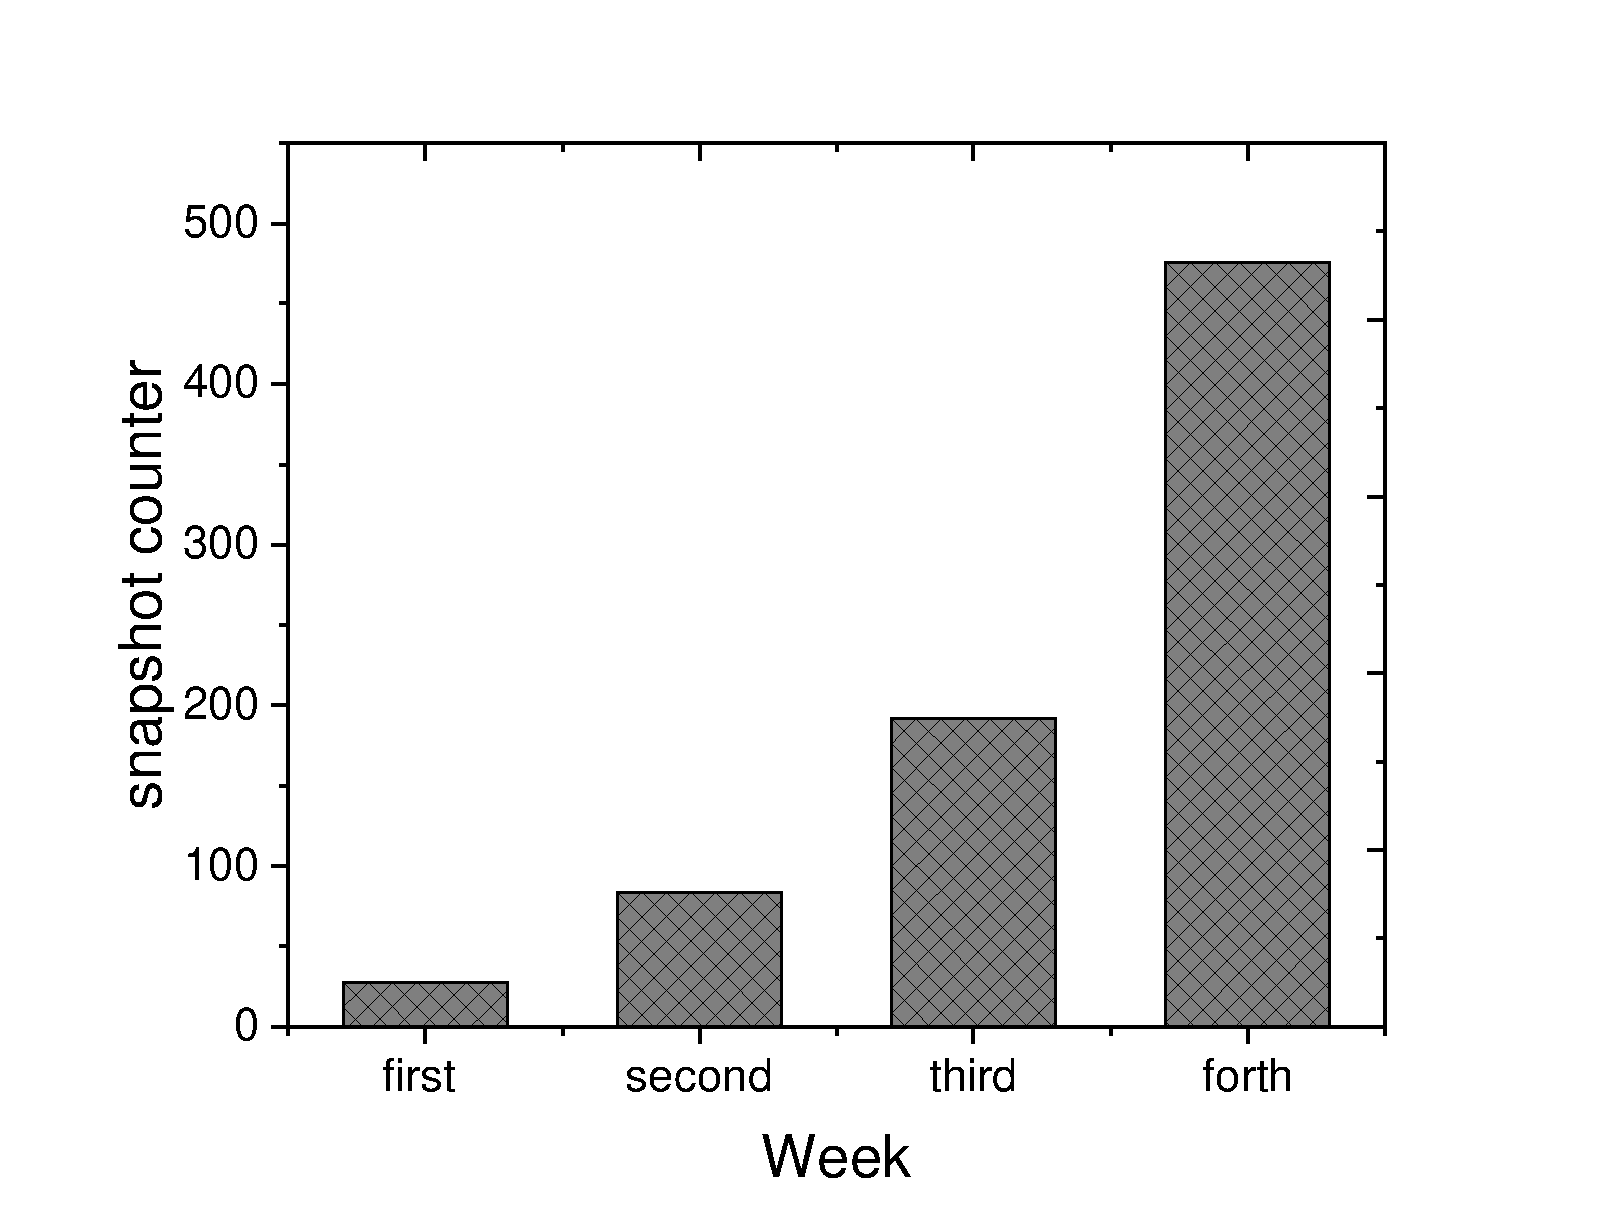
\includegraphics[width=\linewidth]{figures/ceph_pic/ali_counter_workload.pdf} 
		\caption{Snapshot retained distribution} 
		\label{fig:retained_distribution}
	\end{minipage}
	\hfill%
	\begin{minipage}[t]{0.48\linewidth}
		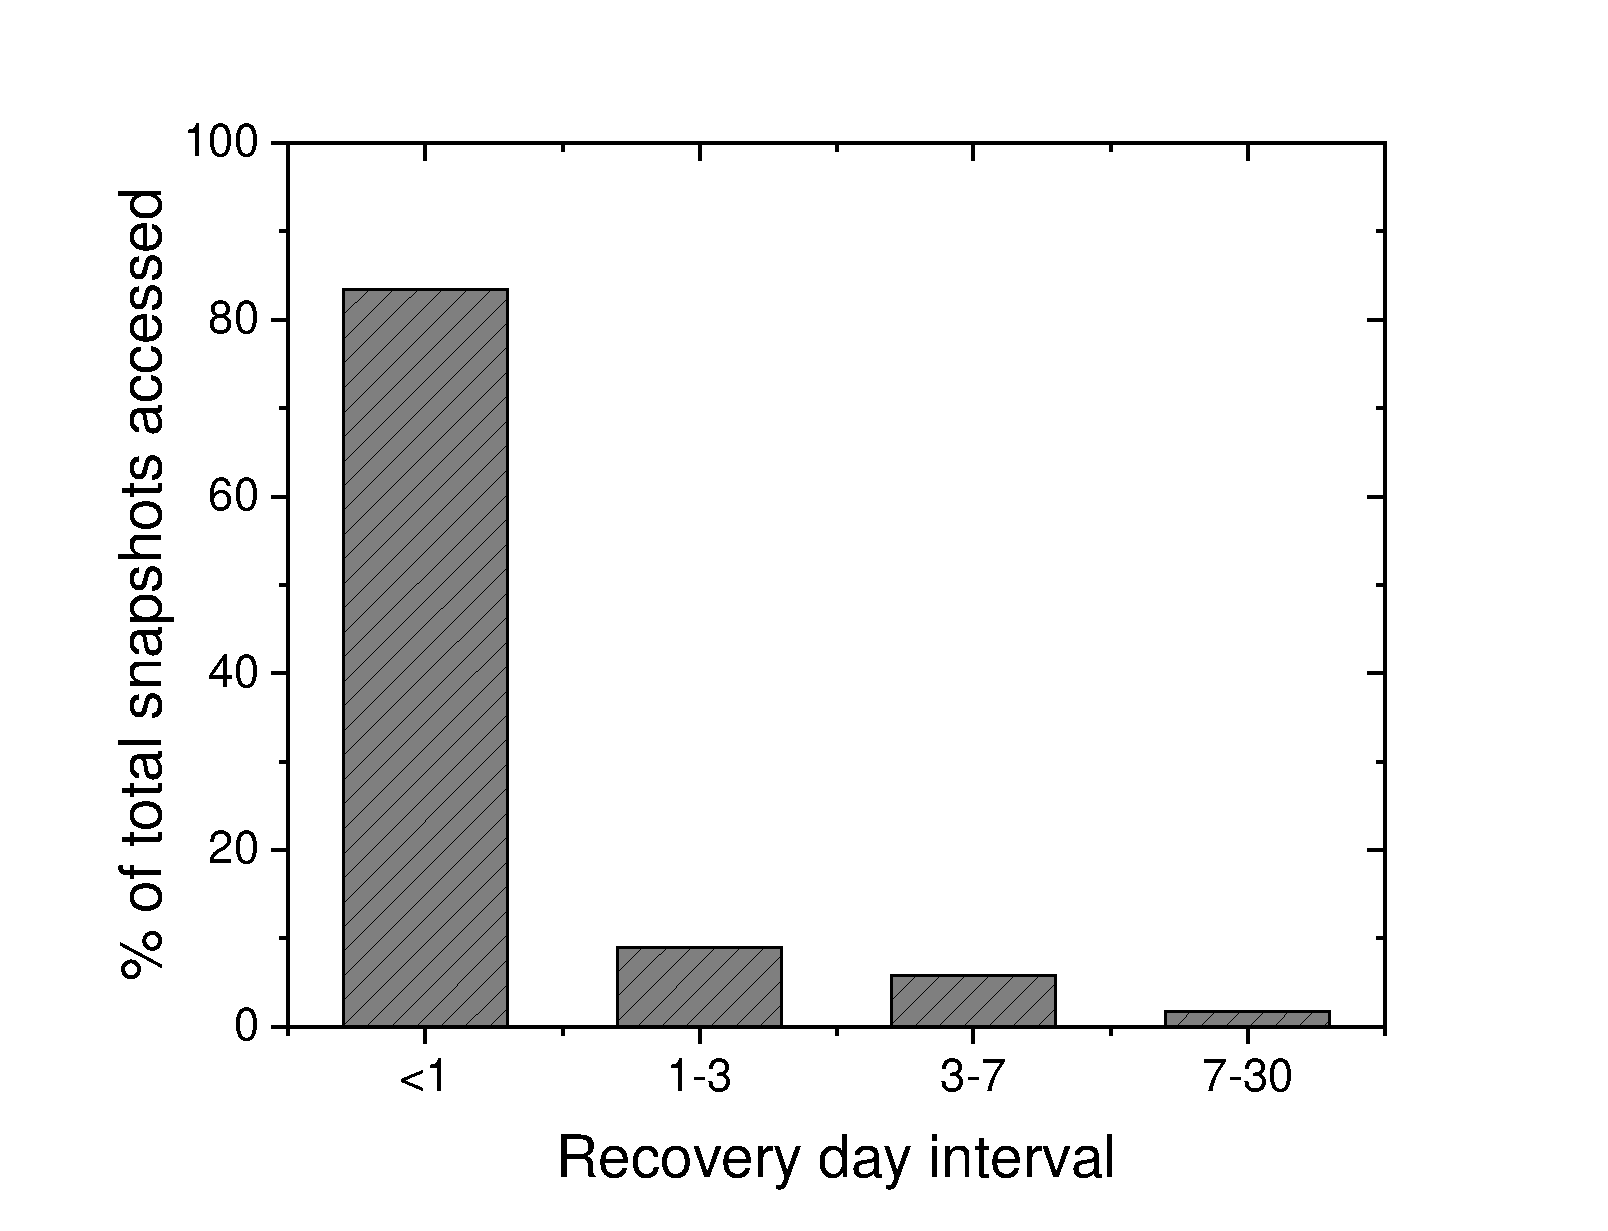
\includegraphics[width=\linewidth]{figures/ceph_pic/ali_percentage_workload.pdf}
		\caption{Snapshot accessed distribution}
		\label{fig:accessed_distribution}
	\end{minipage} 
\end{figure}




\section{Motivation}
\label{Motivation}

\subsection{Fragmentation and Iterative Traversal}
As discussed in Section 2, fragmentation causes serious iterative
traversal in snapshot versions based on the RoW technique. In this
subsection, we analyze the reason of iterative traversal with a typical
example.

\begin{figure}[htp]
	\centering
	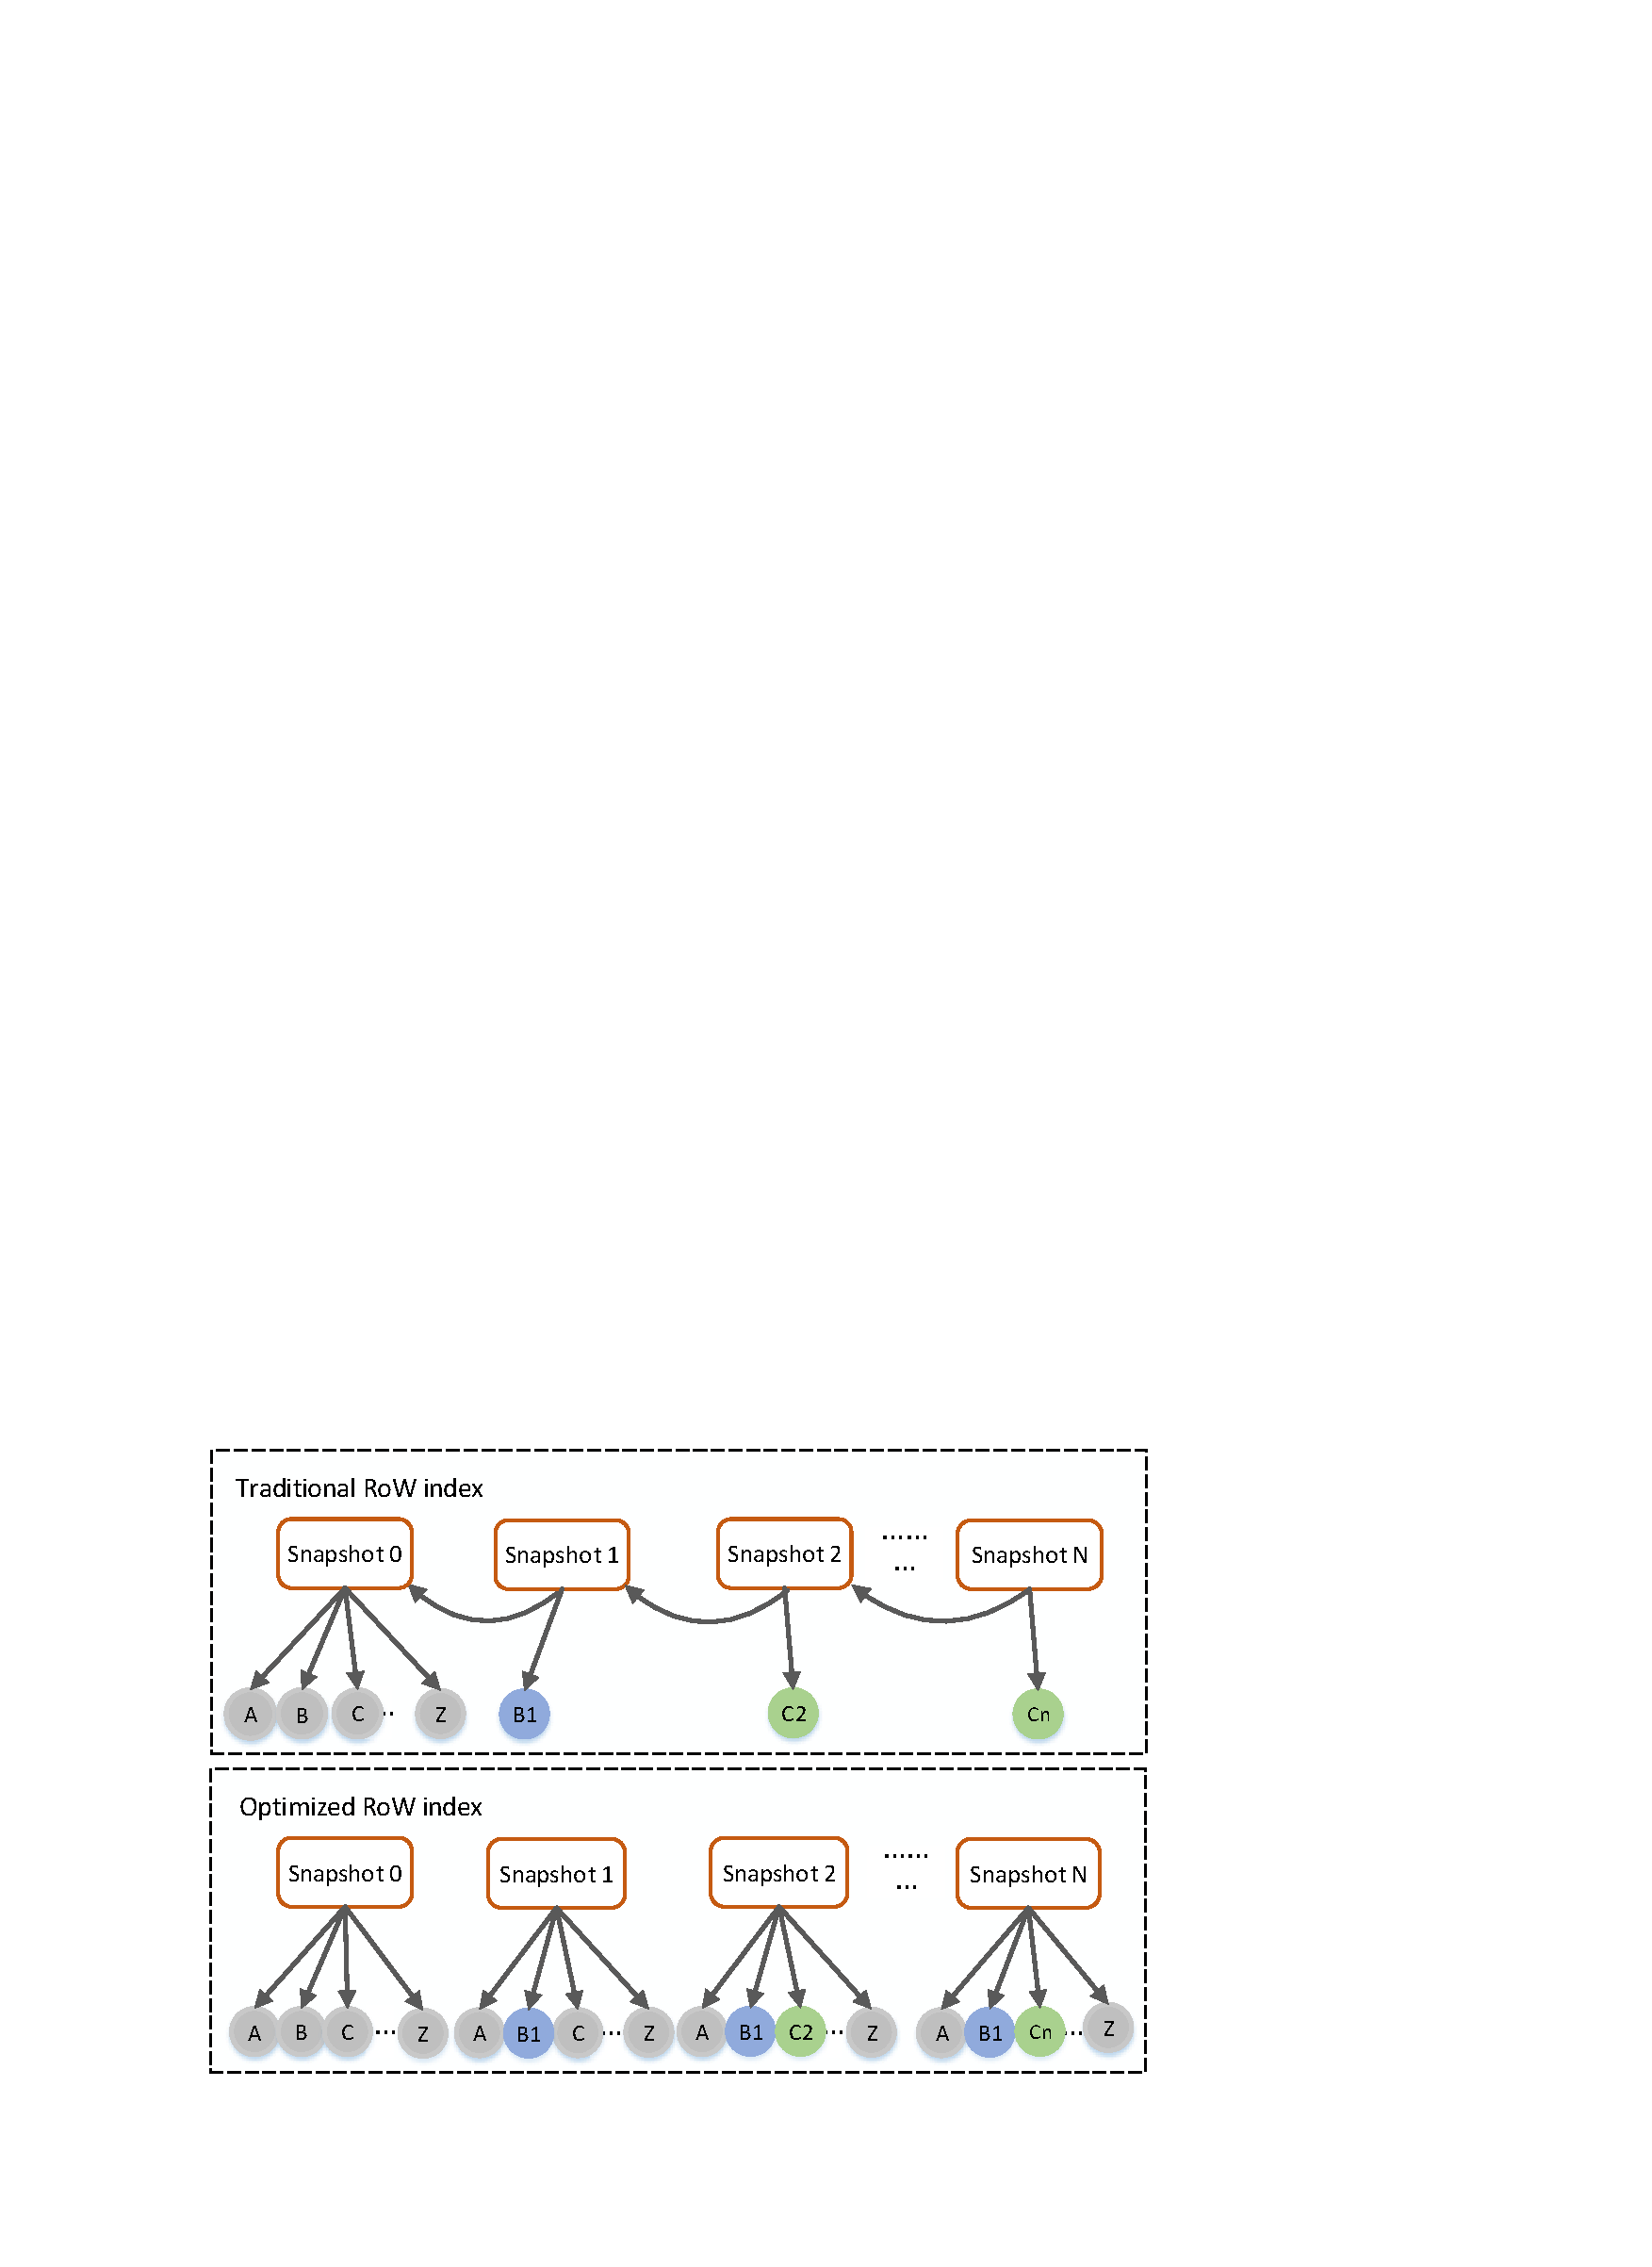
\includegraphics[width=\columnwidth]{figures/ceph_pic/orig_RoW_and_OpRoW.pdf}
	\caption{Example of unbounded traverses to restore snapshots on traditional versus optimized RoW index}
	\label{fig:row-index-vs}
\end{figure}


In traditional RoW, new data blocks are written to the current snapshot, and the snapshot stores a uniform previous snapshot number for unmodified data blocks. During the snapshot recovery phase, the recovery process requires access to other snapshots because the data blocks of the snapshot are scattered in other snapshots rather than only in the current snapshot. The first step in locating an unmodified data block is to verify the destination snapshot, and then check the existence of the data block. As shown in Figure \ref{fig:row-index-vs}, there are \emph{Block A}, \emph{B} until to \emph{Z}. \emph{Block B} is updated in \emph{snapshot 1}, \emph{Block C} is updated in \emph{snapshot 2}. When restoring \emph{snapshot 1}, only \emph{snapshot 0} and \emph{snapshot 1} are verified. However, when restoring \emph{snapshot N}, the recovery process first checks \emph{Block A} in \emph{snapshot N-1}, but \emph{Block A} is not updated in \emph{snapshot N-1},  it has to recall a snapshot iteratively until found in \emph{snapshot 1}. For \emph{Block B}, the same traversal path is required. The recovery latency is affected by the data block fragmentation and the number of snapshots.
With the optimized RoW in Figure \ref{fig:row-index-vs}, the snapshot copies all snapshot numbers for unmodified data blocks at the end of the snapshot period.
However, each snapshot index is a complete tree, which puts significant pressure on the memory capacity of the client node and snapshot loading from the storage cluster due to the snapshot access characteristics.

Amazon EBS \cite{varia2014overview} relieves memory pressure by replacing leaf nodes with regions based on the optimized RoW index.
However, when the fragmentation of the data block increases, the size of the region is dropping while the number is increasing. Thus the index degenerates into the optimized RoW index which significantly boosts the memory usage of the index.

\subsection{Optimal Snapshot Index}
Under the observations and comparisons of existing snapshot indexes, fragmentation caused serious iterative traversal in snapshot versions based on the RoW technique.  
We present an optimal snapshot index namely GSnap, which cuts off the reference by putting the snapshots into the group to eliminate iterative traversal. 

\textbf{An example of GSnap:} For the \emph{snapshot 1}, \emph{2}, \emph{3}, we put them into a group. \emph{Snapshot 1} records the modified data block during the snapshot period, namely \emph{Block B1} and records all unmodified data blocks since it is the first snapshot in this group, thus its index is a complete tree.
The next \emph{snapshot 2}, \emph{3} no longer need to store addresses of the unmodified data blocks any more, and only store \emph{Block C2} and \emph{C3} respectively. When restoring a snapshot, we load the group into memory that means all snapshots in the group are restored, from this observation that the snapshot accessing is usually continuous. The snapshots after this group are also divided into individual groups, which are organized similarly. The rationale behind this is to cut off the reference relationship between two groups while implementing incremental snapshots in a group. Only the snapshots within the group need to be accessed to avoid iterative traversal when looking up the address of a data block.

\begin{figure}[htp]
	\centering
	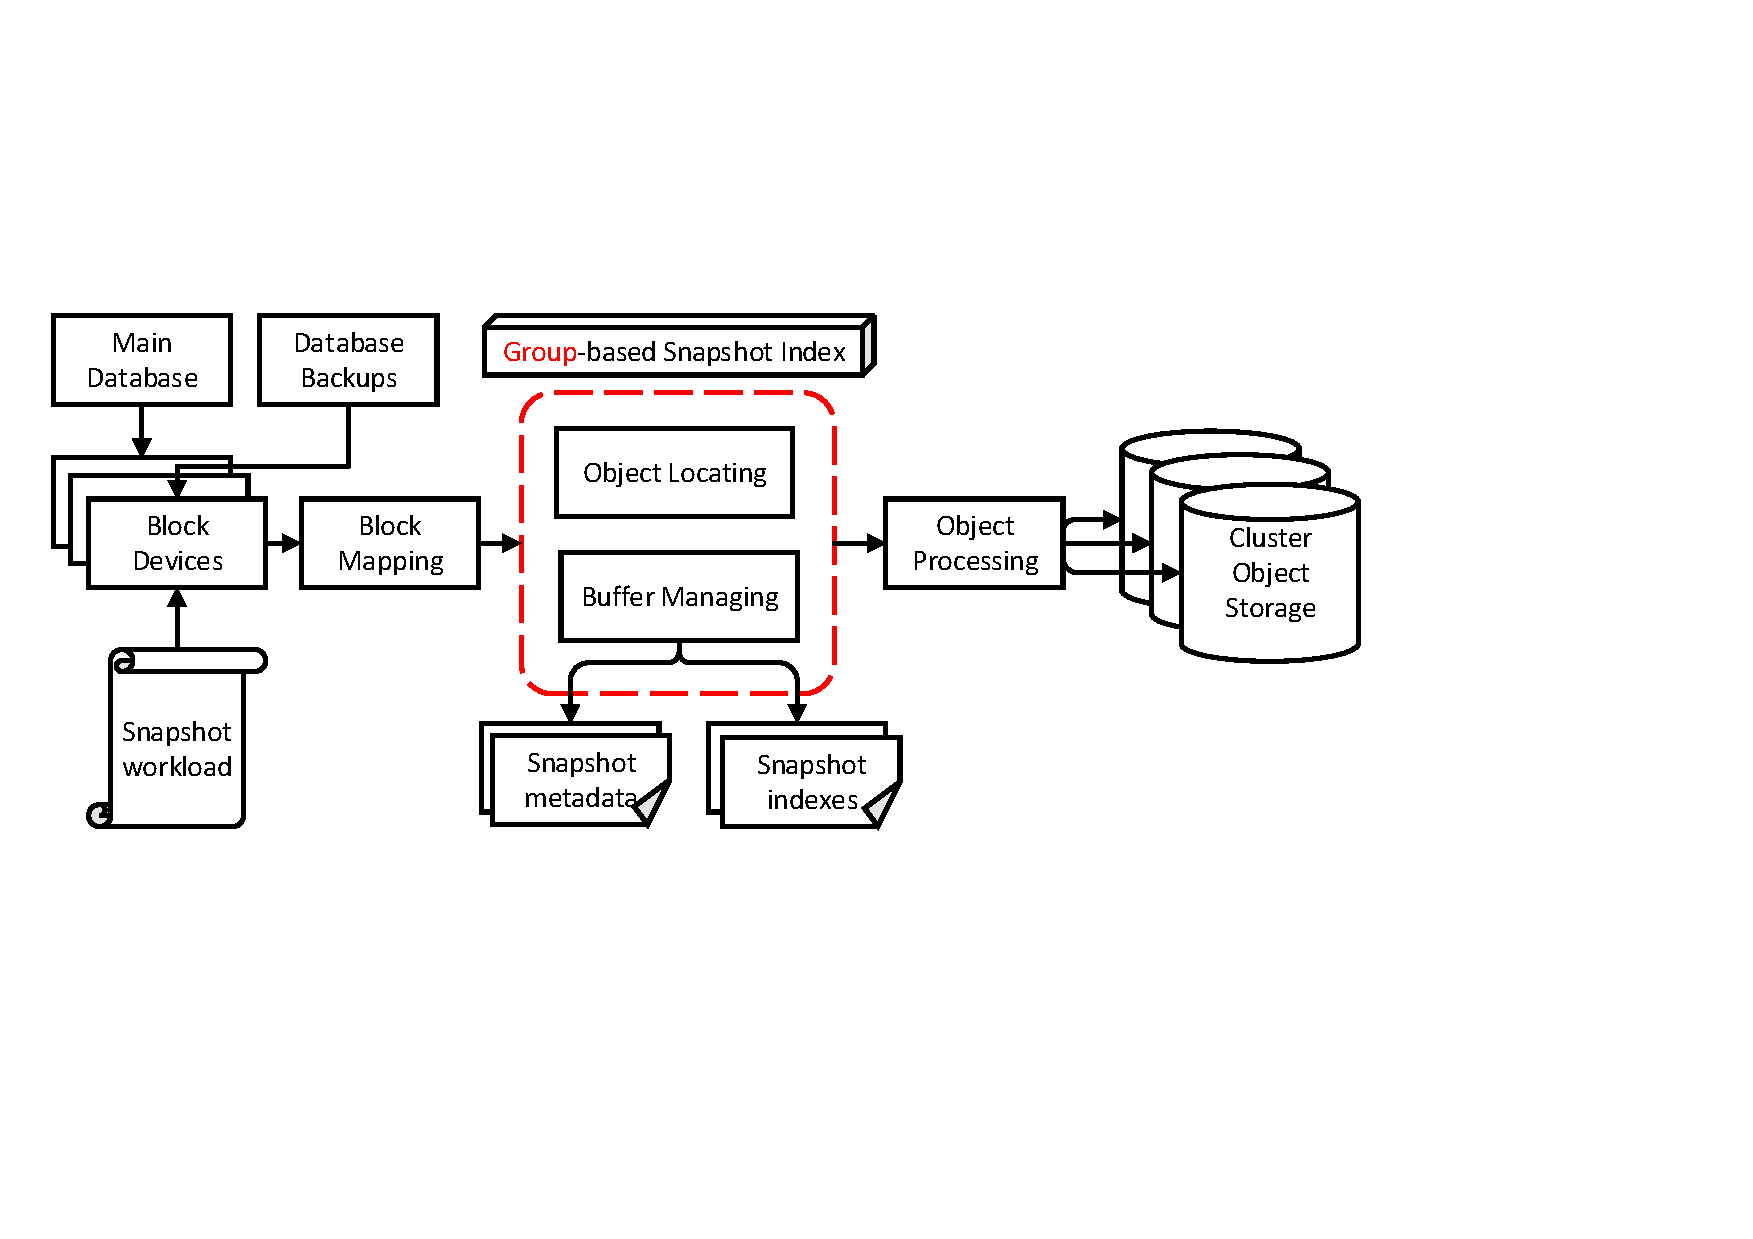
\includegraphics[width=\columnwidth]{figures/ceph_pic/arch_overview.pdf}
	\caption{An overview of GSnap index framework}
	\label{fig:framework}
\end{figure}

\textbf{GSnap framework overview:} GSnap manages the indexes within the group by using two key techniques. The overall workflow of the GSnap framework is shown in Figure \ref{fig:framework}, which includes three key stages: \emph{Block Mapping}, \emph{Indexing}, \emph{Object Processing}.
\begin{figure*}[htp]
	\centering
	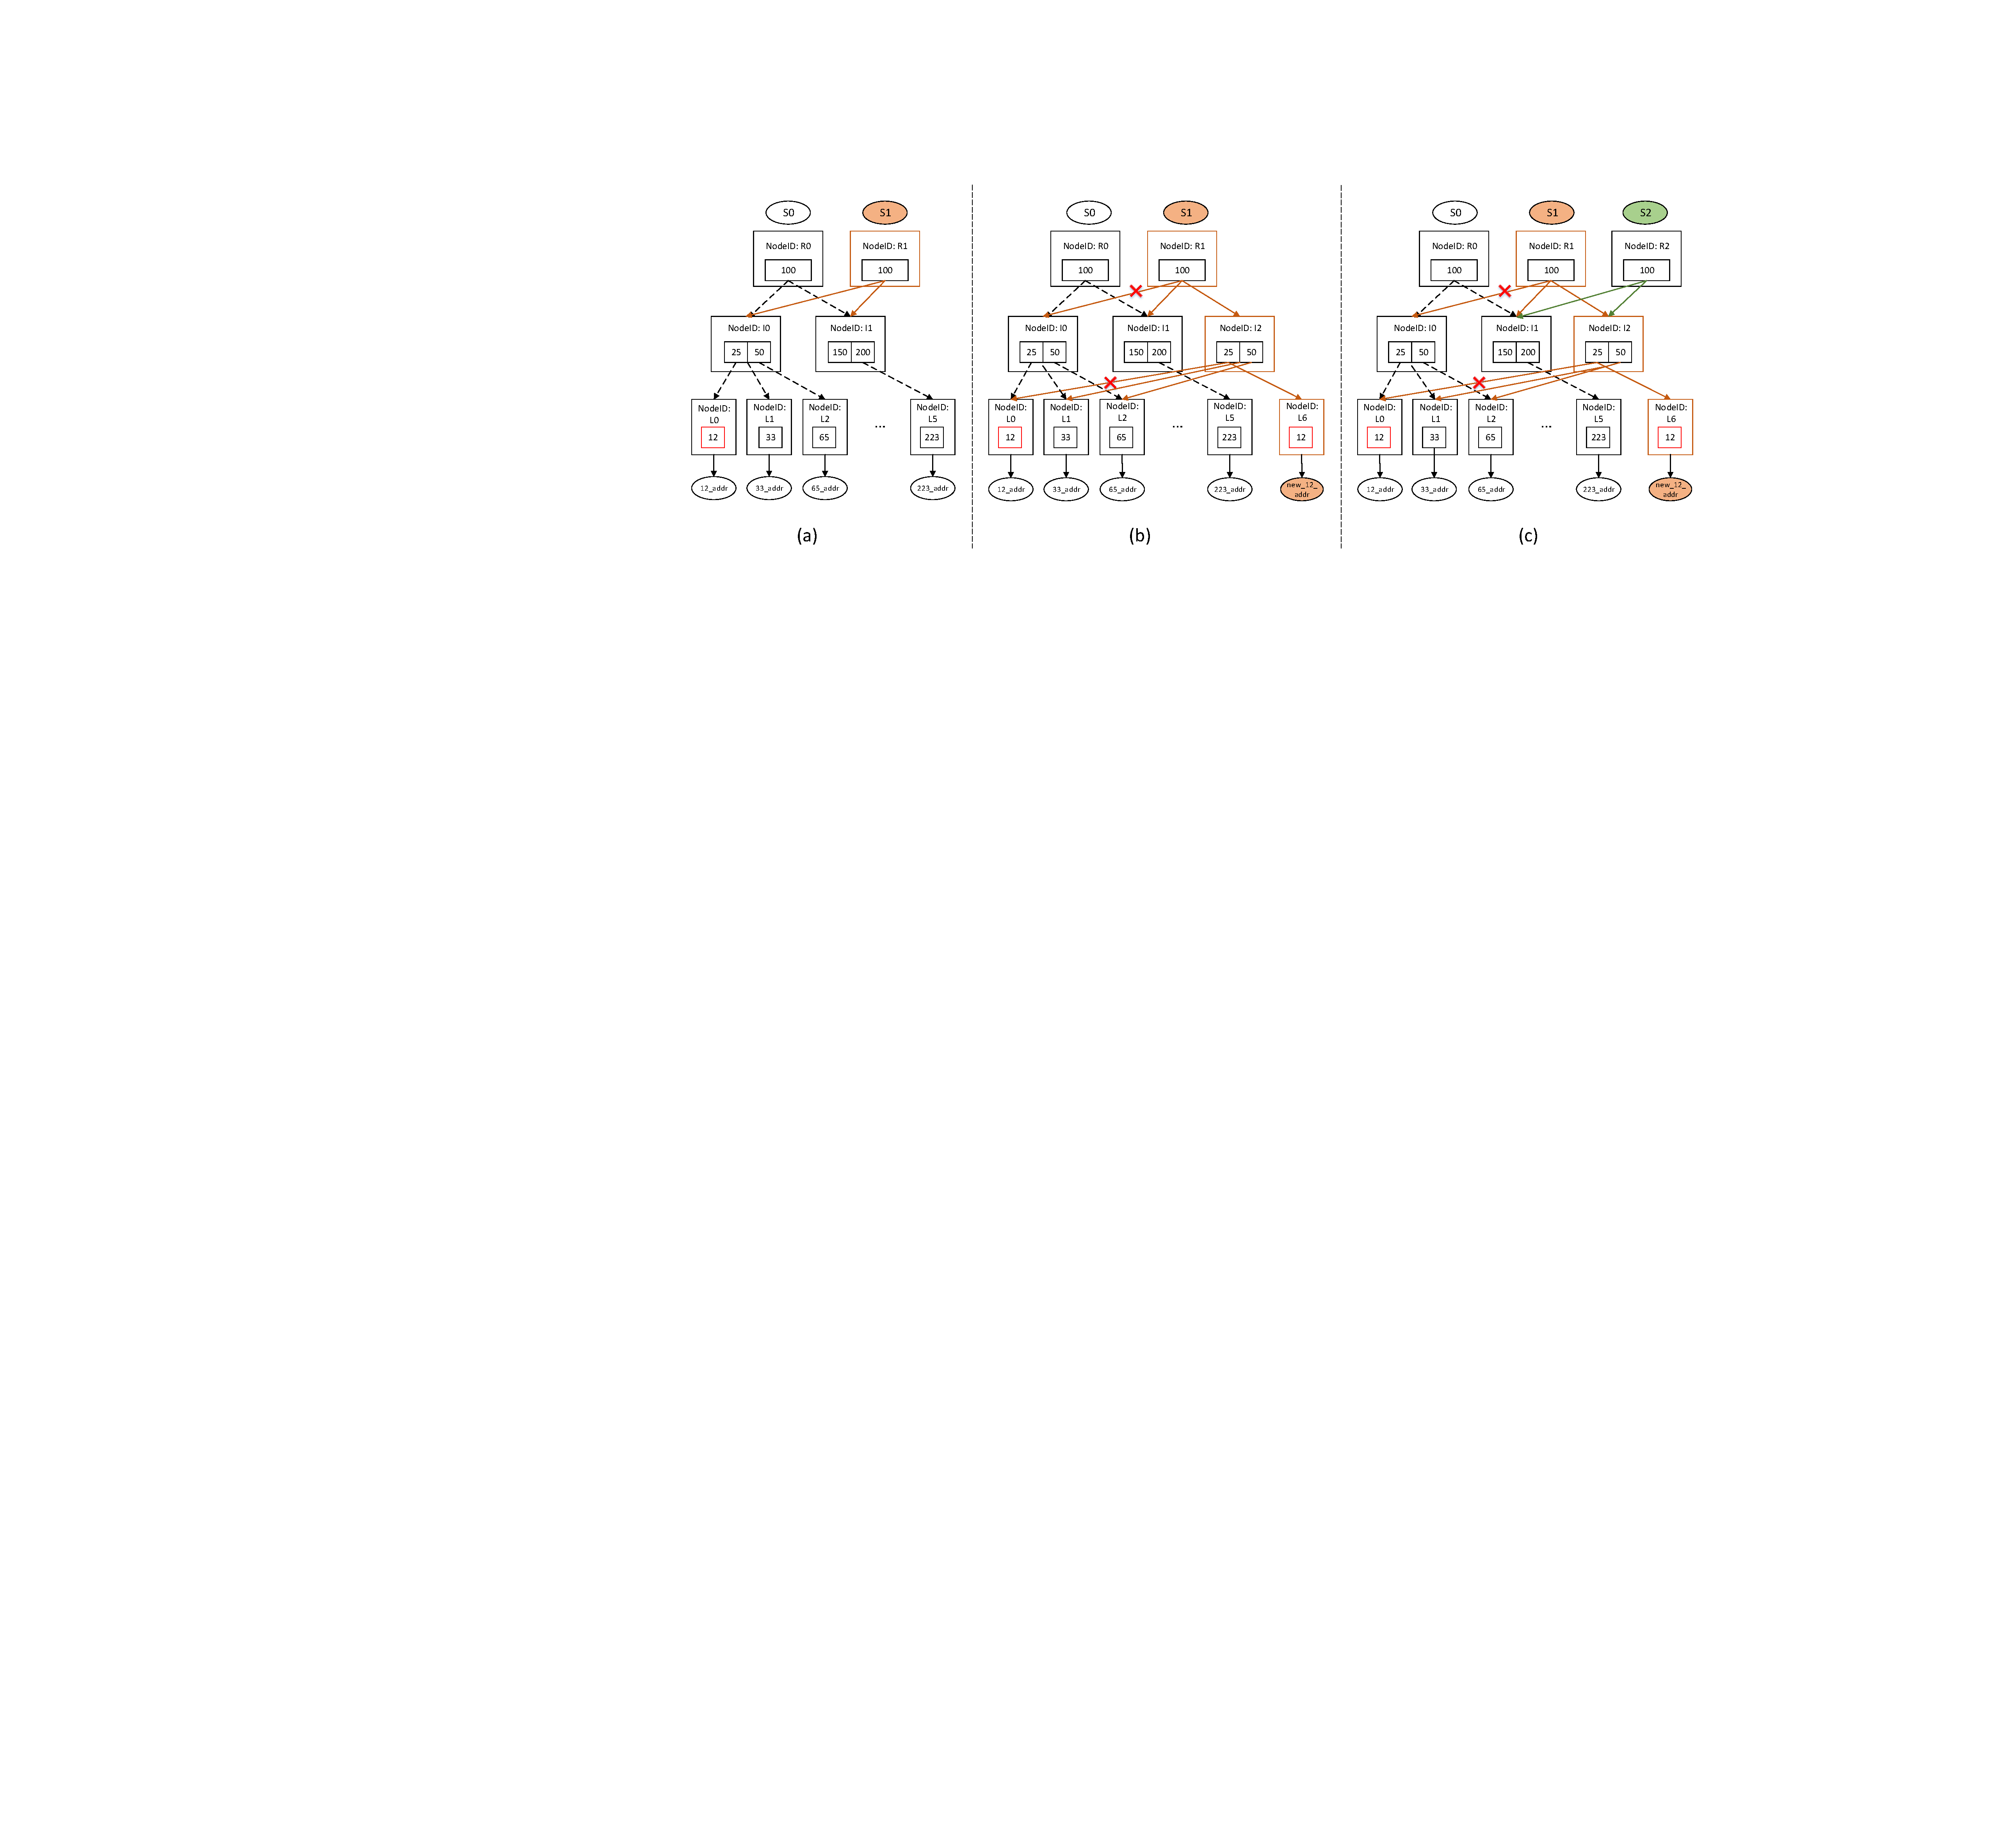
\includegraphics[width=16cm]{figures/ceph_pic/snaptree.pdf}
	\caption{SnapTree: \textbf{(a)} Create S1 snapshot. \textbf{(b)} Block No.12 data write. \textbf{(c)} Create S2 snapshot}
	\label{fig:snaptree}
\end{figure*}
\begin{itemize}
	\item \textbf{Shared-Subtree Indexing(SSI)}. The snapshot index is organized in the B+ tree structure and the leaf nodes store the addresses of the data blocks. SSI shares the internal and leaf nodes among the indexes. Hence, we only need to build and insert nodes when data blocks are modified to maintain that the path from the root node to the leaf node is complete, as detailed in Section \ref{SSI}.
	\item \textbf{Group-Based Dividing(GBD)}. 
	GSnap triggers GBD once the data blocks updated in the group are saturated. GBD initializes the state of the new group to the active and flushes the achieved group to the storage cluster. Specifically, GSnap allocates data block budget and sets the length of the group by Algorithm \ref{algorithm:dividing}, as detailed in Section \ref{GBD}.
\end{itemize}
Block Mapping refers to the read/write requests of the database being mapped to the logical blocks of the block device through the Linux Storage Stack(LSS). The block device can be Rados Block Device(RBD) \cite{weil2006ceph} or Network Block Device(NBD). Indexing accelerates the mapping of logical block numbers to physical blocks. Object Processing indicates that the subsequent requests are processed asynchronously via transactions after the network connection is established with the target object storage node. Write operation requests are duplicated across multiple nodes.
In general, group-based snapshot index consists of two parts, data block locating and cache management. Data block locating works in snapshot accessing and group restoring. 
The cache management loads snapshot indexes based on the access characteristics and adopts the LRU algorithm to swap out the snapshot group, which effectively reduces the index memory overhead.

\textbf{Challenges for GSnap.} Actual snapshot workloads are much more complicated than the example shown in Figure \ref{fig:row-index-vs}, this results in inconsistent update frequency in each snapshot. Then the number of updated data blocks and the length of group are the key factors for taking and restoring snapshots.
The update delay and memory usage of the index are proportional to the number of data blocks, we set the block budget for the latter group based on the block consumption of the former group to reduce memory overhead.
The snapshot group length is still rewarded by the the former group so that ensure the indexes of each group occupy a close memory size for stable snapshot recovery and simple memory management. Besides, as we know from the previous section that users access snapshots continuously, we tend to set the length of the group is equal to the recent average access length of snapshots. We discuss those factors in detail in the next section.


\section{Design and Implementation}
\label{Design}

\subsection{Shared-Subtree Indexing}
\label{SSI}
Snapshots also organize data blocks like the file system through a tree. The addresses of data blocks are stored in the leaf nodes. The root node and internal nodes point to the next level nodes and the key in the node is the ID of the data block. Moreover, we set an ID namely \emph{NodeID} for each node in the tree. 
The index just copies the root node of the last index as the new root node which may share subtrees with other indexes once the user creates a snapshot.
Data blocks shared with the snapshots can not be updated in place when write operations to a block device come.  All writes must be redirected to the new data blocks which created by the current snapshot. The index creates leaf nodes for new data blocks, then checks whether the path from the leaf nodes to the root node is complete. If not, the index duplicates the internal nodes from the previous index, and finally modifies their pointers to redirect to the new leaf nodes. However, the nodes that record unmodified block numbers still point to the prior indexes.  


We show SSI with an example in Figure \ref{fig:snaptree} (a), when the user takes the snapshot \emph{S1}, \emph{S1} just copies the root node from the snapshot tree \emph{S0}, as the new root node namely \emph{R1}, and \emph{R1} points to the internal nodes \emph{I0} and \emph{I1}. 
Figure \ref{fig:snaptree} (b) shows that block \emph{No.12}, whose address is recorded by the leaf node \emph{L0}, is updated in the snapshot period. Firstly, \emph{S1} creates a new leaf node \emph{L6} and stores the address of the new block, then checks whether the path from the root node \emph{R1} to the target leaf node \emph{L6} is complete. If not, \emph{S1} copies all internal nodes from \emph{R1} to \emph{L0}, and then changes the pointers to redirect to those new nodes. The root node \emph{R1} points to internal node \emph{I0} and changes to point to new internal node \emph{I2}, then \emph{I2} redirects to leaf node \emph{L6} instead of \emph{L0}. In the same way, the root node \emph{R2} points to internal nodes \emph{I1} and \emph{I2} when taking the \emph{S2} snapshot.

There are two advantages of the shared subtree structure. Firstly, the memory footprint occupied by the tree is proportional to the number of updated data blocks in this snapshot, which means the memory footprint is small because most snapshots are not updated frequently as mentioned in Section \ref{Characters} and the index redundancy is reduced by only saving one copy of the address. 
Secondly, the subtree sharing among snapshots makes locating the leaf nodes on any snaptree in a constant time. The reason is that the number of hops to locate a leaf node is the same as the height of the tree.

\subsection{Group-Based Dividing}
\label{GBD}
In this subsection, we introduce the Group-Based Dividing method, which is designed to cut off the snapshot index dependency and establish snapshot recovery granularity.
There are two stages in GBD, the snapshotting stage and the dividing stage. 
In the snapshotting phase, the snapshot indexes generated in the group are partial trees. Besides, the state of the last index is \textbf{active} while others are \textbf{achieved}.  In the dividing phase, the first snapshot index generated in the next group is a complete tree. The state transformation between the two stages is determined by the update ratio of the snapshots in the group and the latest average continuous access interval. 

\textbf{Snapshotting stage.} In this stage, the system only copies the root node of the previous snapshot index for the new snapshot index. The new root node points to all internal nodes of the previous index and the number of snapshots in the group $S$ plus 1.
Besides, the \emph{Is\_Created} flag of all internal nodes in the index are reset to false, which implies that no nodes are created in the index yet.
As shown in the Figure \ref{fig:snapshotgroup_devide}, when the data blocks updated dose not reached the saturation, the snapshot index $S_1$ only copies one root node, the reference of all leaf nodes in previous index is incremented by 1. 
At the same time the previous index status is converted to \textbf{achieved}, and the current snapshot index status is \textbf{active}, which means all writes are updated in the current snapshot and only the current index could be modified during the period. 
We collect the update ratio of the former group $P$ after the group state is changed.
Once a data block is updated, the block counter $O$ recorded in group increase by 1 and the \emph{Is\_Created} flag of the new added internal nodes are set to true.


\textbf{Dividing stage.} When the number of snapshots $S$ or the block counter $O$ in the group reaches the threshold, the group state transforms into the dividing state. $S$ and $O$ are factors to trade off the recovery speed and memory overhead, they will be discussed in Section \ref{section:Recovery model}. Figure \ref{fig:snapshotgroup_devide} shows that the snapshot index $S_n$ traverses all the leaf nodes of $S_{n-1}$ and constructs a complete tree. Since traversing the leaf nodes only needs to access the root node of the last snapshot index and the number of hops is fixed, which speeds up the construction of the tree.
GSnap allocates the block budget and set group length to the latter group based on the block consumption of the former group and the latest average continuous access snapshot length namely $L^\ast$. 
We constrain the continuously accessed snapshots in a group and adjust the size of the group based on the update ratio of snapshots.
As shown in Algorithm \ref{algorithm:dividing}, GSnap compares the block budget $O^\ast$ with the block counter $O$ and set the block and group length budget of the latter group. If the block counter $O$ equals the block budget $O^\ast$, that means the block budget has been exhausted and the length of the group has not reached the threshold. GSnap rewards the latter group with the same update ratio and does not change the group length budget. The latter group is punished if the block budget is not used up, and the length budget is decreased to $p$, and $p$ is the punish factor. In addition, we take the maximum value between $S_{n+1}$ and the average continuous access length  $L^\ast$ to cover the snapshot set.


\begin{algorithm}[htp]
	\caption{GSnap Index Group Dividing}
	\label{algorithm:dividing}
	\KwIn{$L^\ast$-The latest average continuous access snapshot length;
		$O_n$-The max number of modified objects in the n-th group;
		$S_n$-The max number of snapshots in the n-th group;
	}
	\KwOut{$SC_n^\ast$-A set which stores pairs from snapshot to modified block count;
		$O_{n+1}^\ast$-The object budget in the (n+1)-th group;
		$S_{n+1}^\ast$-The snapshot budget for the (n+1)-th group;}
	
	init $O_n$, $P_n$, $SC_n$;\\
	\While{$O_n^\ast$> $O_n$  $\&\&$ $S^\ast$.siz><$S_n$}{
		do taking snapshot and updating index;\\
		$SC_n^\ast$.insert(snapid, count);\\
		$O_n$ += count;\\
		update $P_n$;\\
	}
	\eIf{$O_n$ $\geq$ $O_n^\ast$}  
	{
		$S_{n+1}^\ast=\max(S_{n}, L^\ast)$;         // length reward \\ 
	}
	{
		$S_{n+1}^\ast=\max(p\times S_{n}, L^\ast)$;         // length punish\\
		
	}
	\hspace*{0.2in} split the group, and transform achieved group; \\
	\hspace*{0.2in} $O_{n+1}=S_{n+1} \times P_n$;\\
	return $O_{n+1}^\ast$, $SC_n^\ast$, $S_{n+1}^\ast$;\
\end{algorithm}



\begin{figure}[htp]
	\centering
	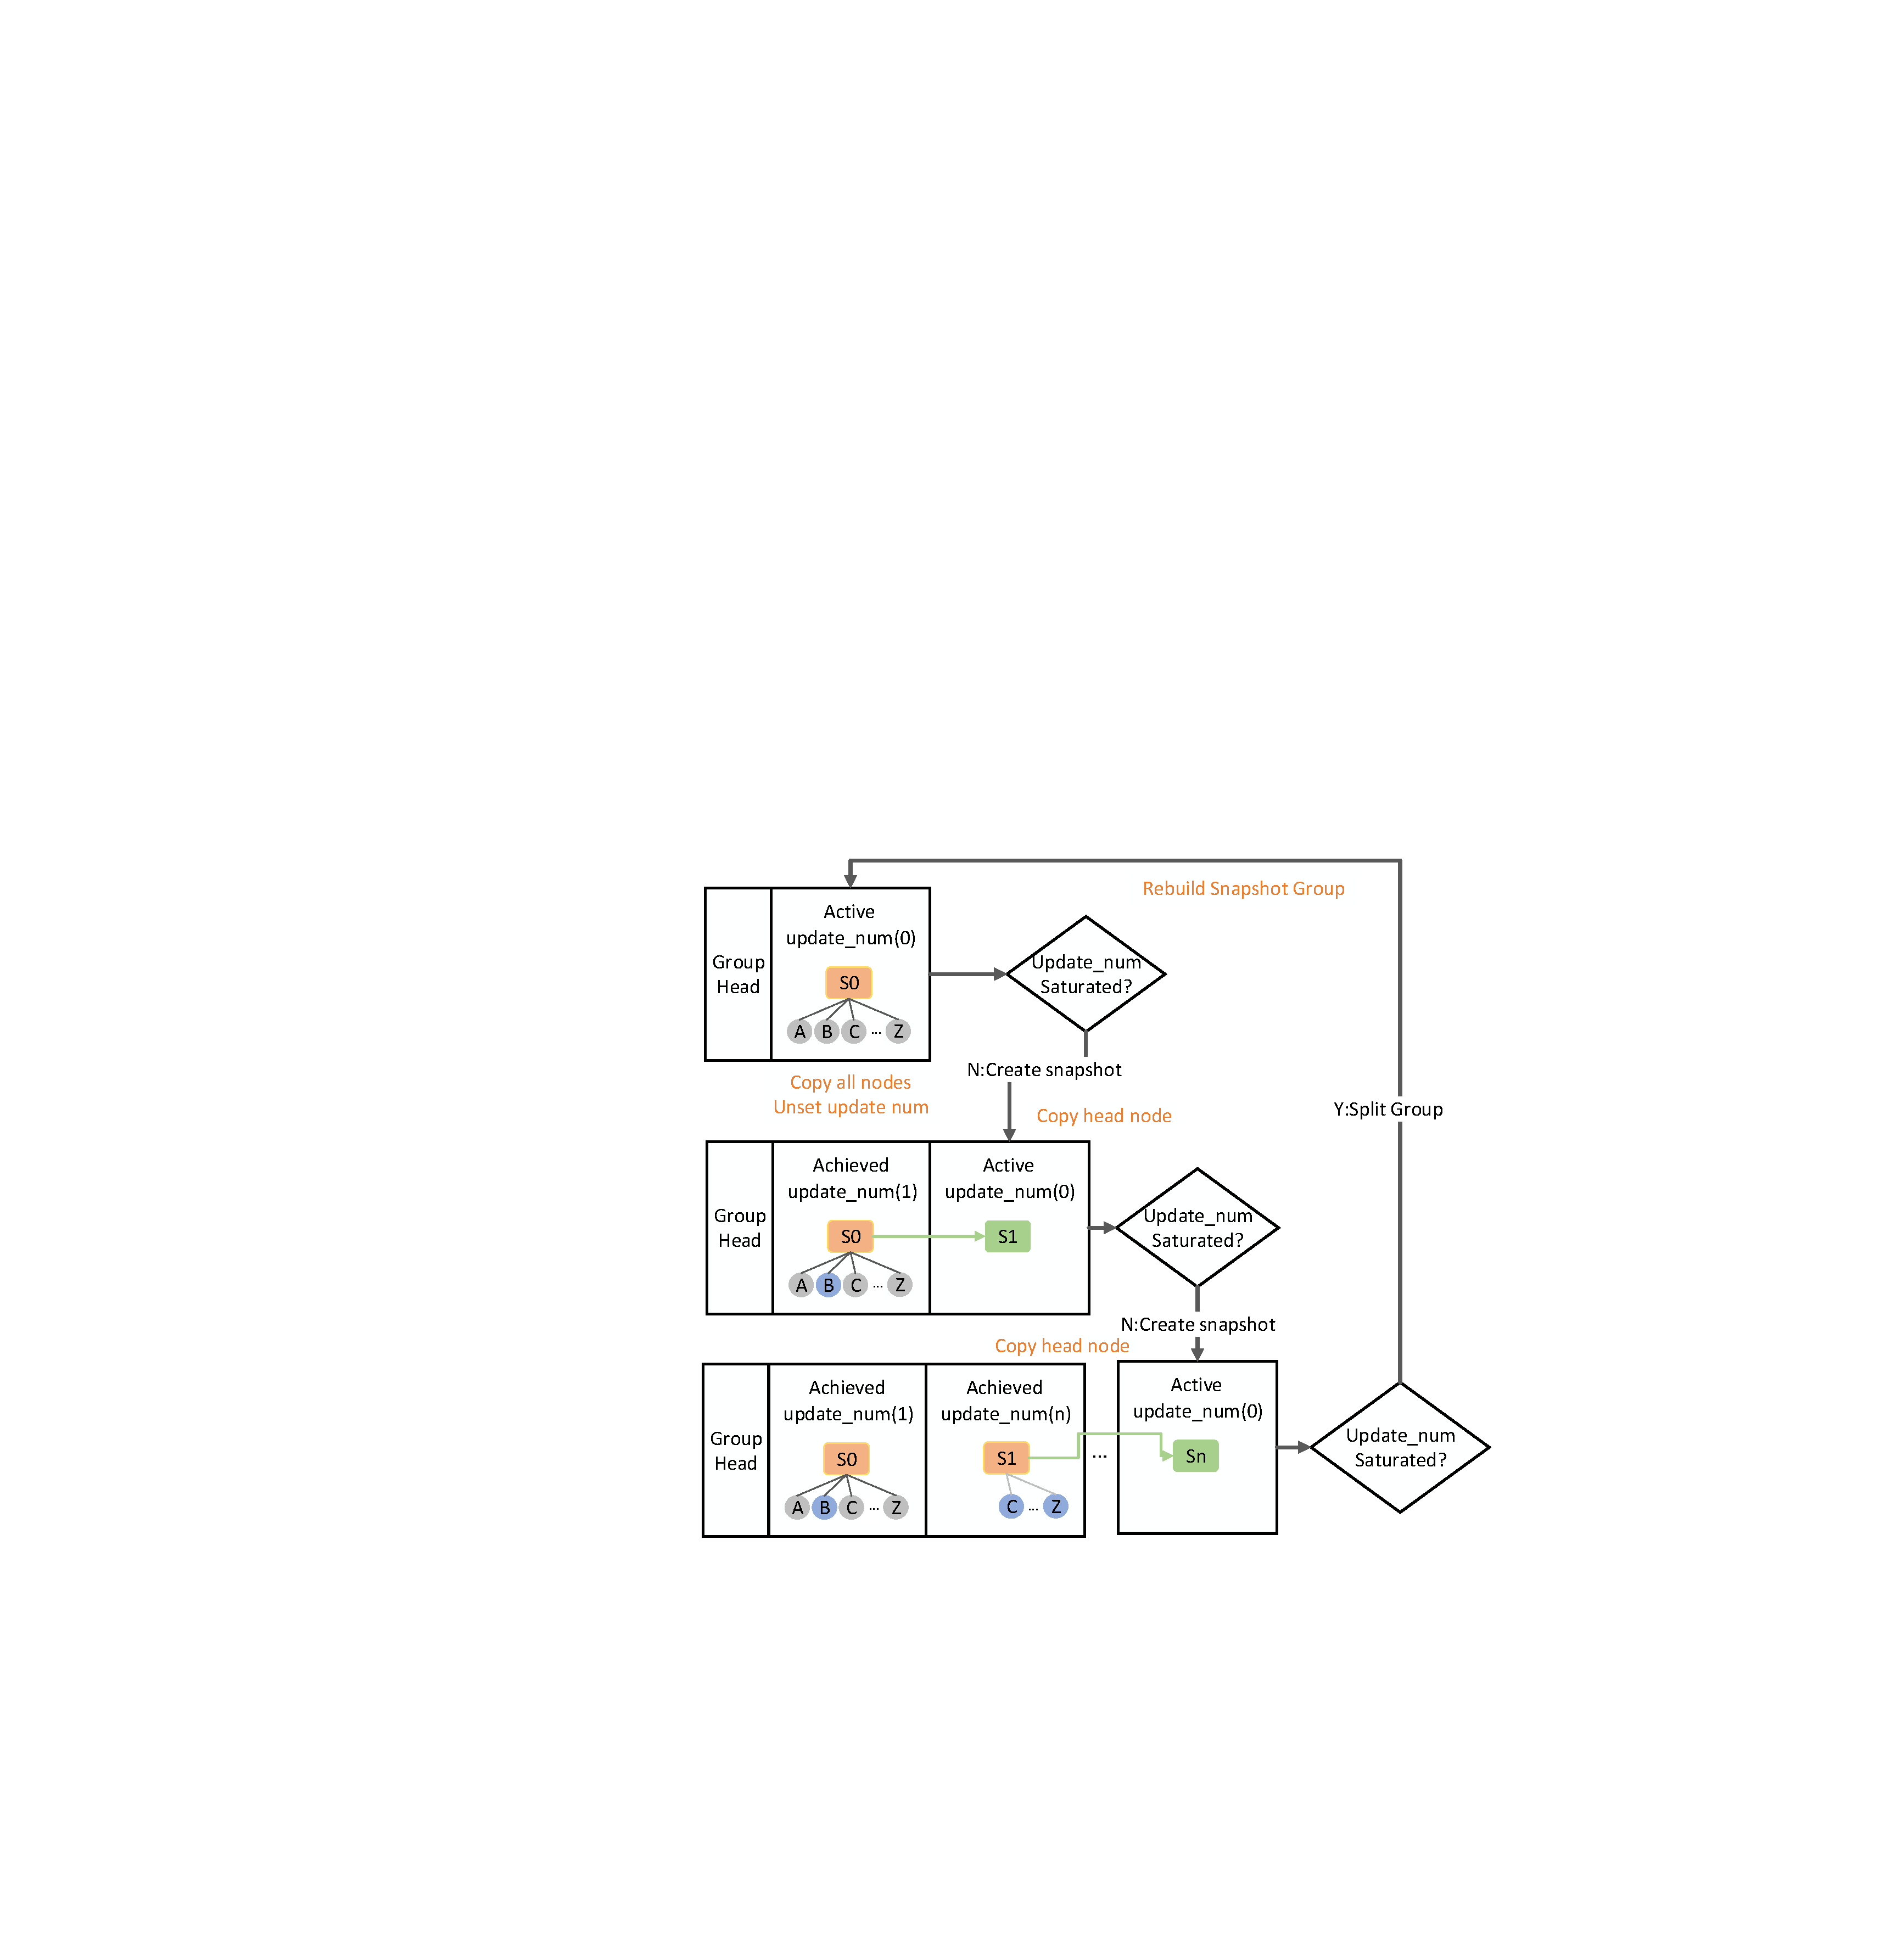
\includegraphics[width=\columnwidth]{figures/ceph_pic/group_divide.pdf}
	\caption{An example of GSnap index division}
	\label{fig:snapshotgroup_devide}
\end{figure}
\vspace{-0.3cm}

\subsection{Cache Management of GSnap}
In this subsection, we introduce how the GSnap index guides the access to the snapshot data block and cache management of the client host.

GSnap uses the shared memory to cache the snapshot index, which is appropriate for interprocess communication. And the user could adjust the shared memory size to accommodate the snapshot size and access frequency by the profile.
When mounting a block device, a daemon process is started in the system for data block locating and index cache management.
As shown in the Figure \ref{fig:cache_managment}, the daemon process allocates memory and initializes \emph{SM\_Admin} and \emph{Snap\_Admin}. \emph{SM\_Admin} is responsible for the expansion of shared memory, which allocates memory segments to the group index and adopts LRU replacement algorithm to swap out the least recently accessed group index. \emph{Snap\_Admin} is responsible for locating and loading the snapshot groups.
At the same time, the snapshot index in the latest group \emph{Latest\_Group} is copied from the storage node to the shared memory, which refers to the snapshot index that has not yet formed a group.

When accessing the snapshot set, the daemon process checks whether the set has been loaded into memory. As shown in Algorithm \ref{algorithm:locate}, \emph{Snap\_Admin} compares the snapshot set $AS$ with the group set $GS$ that already loaded into memory.
If $coverd$ is true and $LS$ is empty, target snapshot set indexes have been loaded into memory. $LS$ contains all the snapshot segments which are needed to be loaded.
Otherwise the daemon process traverses $LS$ and $Group\_Set$ to determine the groups need to be loaded. Finally, \emph{Snap\_Admin} finds the addresses of the index groups in $Group\_Addr\_Set$, and actively load them from the cluster into the shared memory.
We use $Group\_Access\_Counter$ to count the number of accesses of the snapshot groups. Once the shared memory is not enough, we adopt a simple LRU algorithm to swap out the least recently accessed index group, and the granularity of swap out is the group instead of the snapshot.

\begin{algorithm}[htbp]
	\caption{Index Group Checking}
	\label{algorithm:locate}
	\KwIn{$GS$-A sorted set includes all pairs from group start to end snapshot id, and groups have been loaded into memory;
		$AS$-The pair of snapshots to be accessed, including the start to end snapshot id;
		
	}
	\KwOut{$covered$-Whether to cover;
		$LS$- A linked list includes all snapshot segments need to load, including the start to end snapshot id;
	}
	
	init $covered$, $AS$, rear=$GS$.size;\\
	\eIf{$GS(0).first \leq AS.first $ \&\& $ AS.second\leq GS(rear).second$}
	{
		\ForEach{LP in GS}{
			\If{$LP.first \leq AP.first$ \&\& $LP.second \geq AP.second$ }{
					$coverd$ = true;\\
						break;\\
			}	
		\eIf{$LP.first \geq AP.first$ \&\& $LP.second \leq AP.second$}{
			$LS$.append($AS.first$, $LP.first$);\\
			$LS$.append($LP.second$,$ AS.second$);\\
		}{
		
		$LS$.append(max($AS.second$, $LP.first$), max($AS.first$, $LP.second$));
	}
			
		}
	
	}
	{
		$LS$.append(uncovered set);\\
		}
	return $coverd$, $LS$;
\end{algorithm}

\begin{figure}[htbp]
	\centering
	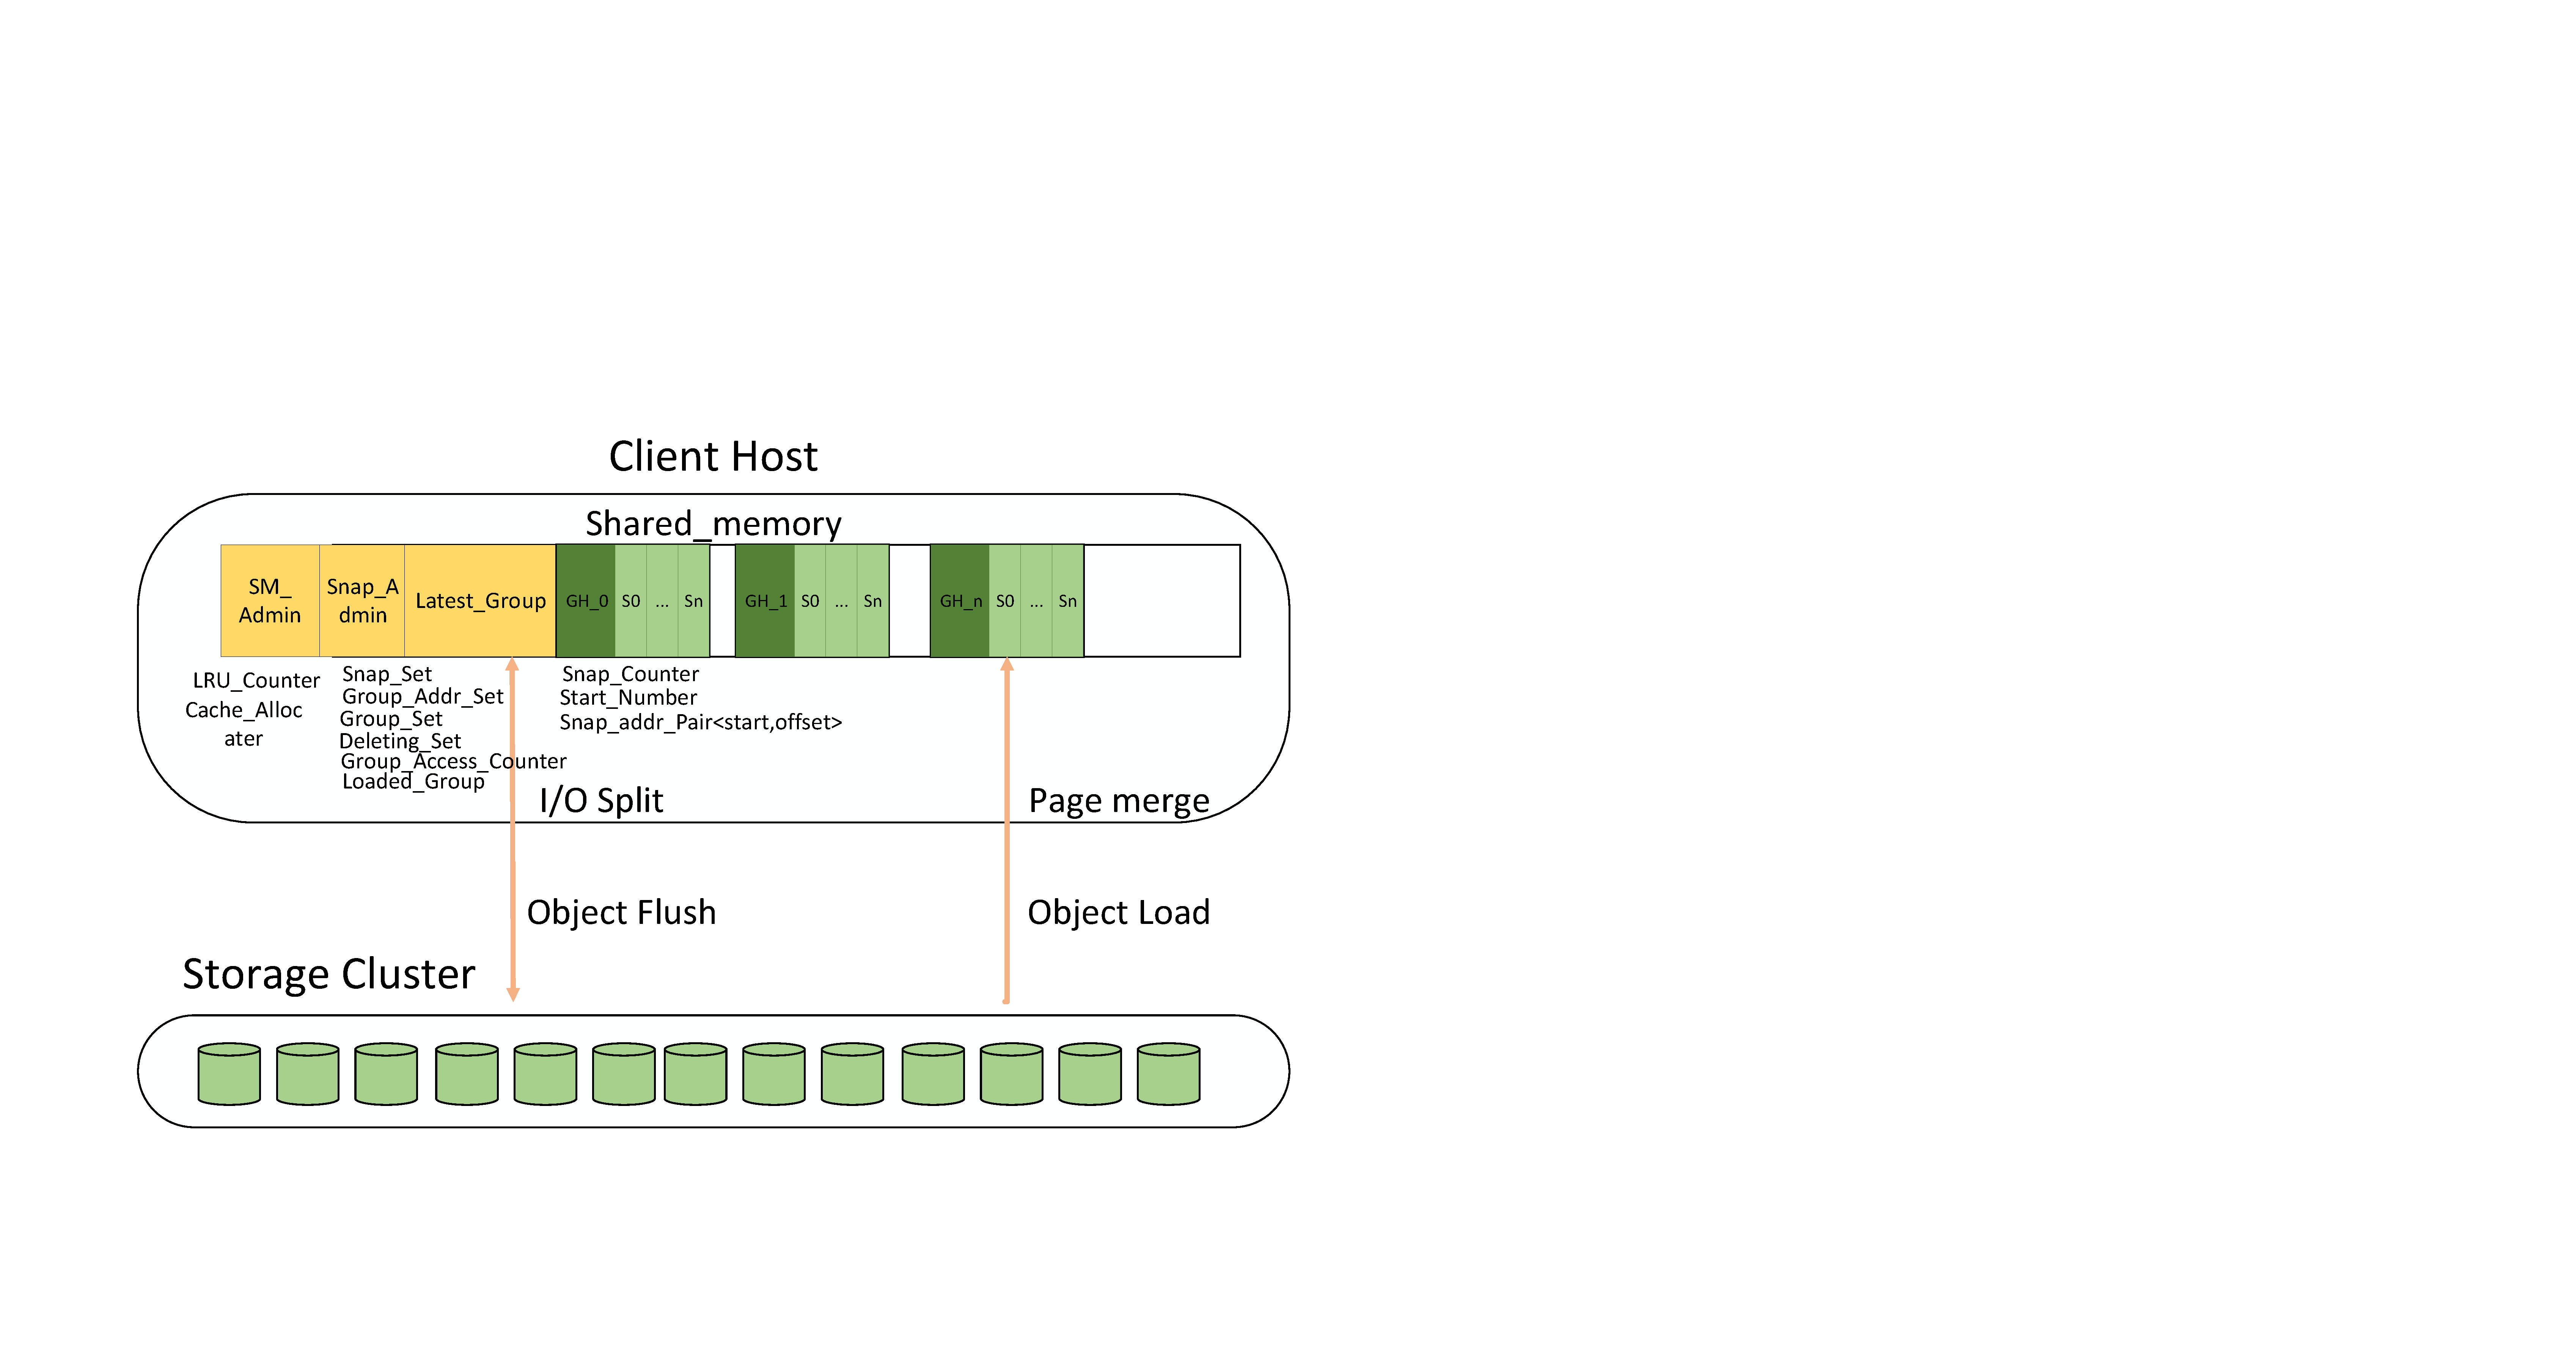
\includegraphics[width=\columnwidth]{figures/ceph_pic/cache_managment.pdf}
	\caption{Cache management of GSnap index on client host}
	\label{fig:cache_managment}
\end{figure}

\subsection{GSnap Recovery Model and Analysis}
\label{section:Recovery model}
In this subsection, we theoretically analyze and compare GSnap recovery with the traditional and optimized indexes, abbreviated as T-index and O-index, from two perspectives: the time cost of building an index and the memory overhead. We also determine the number of snapshots $S$ and the object budget $O$ based on the benefit.

When recovering and cloning a snapshot, the system loads snapshot group and constructs the index in memory first. However, due to the sharing of subtrees, the prerequisite for the construction of the current snapshot tree is that all the subtrees that depend on have been constructed.
The dependence chain length can not be ignored since the low update frequency of the data blocks and update skew in the snapshot. Further, the memory footprint is cautious that impossible to construct all snapshot indexes. 
Therefore, we compare the existing indexes from these two perspectives respectively.

\begin{table}[htbp]
	\centering
	\caption{Group recovery notation definition.}
	\label{table:paramters}
	\resizebox{\columnwidth}{30mm}{
		\begin{tabular}{cc}
			\hline
			Notation & Description                                                  \\ \hline
			$D$        & The size of the block device (GB)                             \\ \hline
			$O_d$        & The object size of the block device (KB)                             \\ \hline
			$r$        & The longest snapshot interval with reference relationship                  \\ \hline
			$P$        & The average update ratio of snapshots                        \\ \hline
			$B$        & The network bandwidth of the storage cluster (Gbps)                 \\ \hline
			$T_a$        & The time cost of accessing memory, about 100 ns                         \\ \hline
			$T_r$       & The time cost of restoring a snapshot                                  \\ \hline
			$M_r$       & The memory overhead of restoring a snapshot                                 \\ \hline
			$M_c$       & The memory consumption of a compete tree                                 \\ \hline
			$M_p$       & The memory consumption of a partial tree                                 \\ \hline
			$T_t$       & The transmission time of each data block                     \\ \hline
			$T_i$       & The average time to insert a node in the snapshot index tree \\ \hline
			$T_l$       & The average time to locate a leaf node                         \\ \hline
			$O$       & The max number of modified objects in a group                          \\ \hline
			$S$       & The max number of snapshot in a group                        \\ \hline
		\end{tabular}
	}
\end{table}

\textbf{Time overhead.} Time overhead refers to the time span in which snapshot could provide services when accessing a certain snapshot. At the stage, the snapshot index is loaded into the memory and the data blocks are still in the physical cluster. We ignore the latency of the access request from the application layer. Even if the delay of the T-index and O-index is higher than the GSnap in loop access requests. We also limit the snapshot recovery to within a group rather than across groups for simplicity. So we have the following equation to define the latency and memory overhead of restoring a snapshot. It may consist of three parts: \ding{172}transform the index blocks from the cluster to the client node; \ding{173}construct the tree and insert  the addresses of all data blocks; \ding{174}locate all leaf nodes when coping nodes to construct a complete tree from the former index. The respective latency of the three stages are:

\begin{small}
	\begin{equation}
		\begin{split}
			T_t&=\frac{1}{32 \times B} \\
			%		T_i > T_l&= O(\log_2(n))  \\
			T_i > T_l&= 8\times \log_2(\frac{D}{O_d})\times T_a \\
		\end{split}
	\end{equation}
\end{small}
\vspace{-0.2cm}

The O-index and GSnap contain traverse overhead because they may construct the complete tree. The time overhead of those indexes during the snapshot restoration is as follows:

\vspace{-0.2cm}
\begin{small}
	\begin{equation}
		\begin{split}
			T_r(T) &= \frac{D}{4}\times(r+1)\times T_t+ 256\times \frac{D}{O_d} \times p \times(r+1) \times T_i\\
			T_r(O) &= \frac{D}{4}\times T_t+ 256\times \frac{D}{O_d} \times (T_i + T_l)\\
			T_r(G) &= \frac{D}{4}\times(s)\times T_t+ 256\times \frac{D}{O_d} \times (1+(s -1)\times p) \times \\
			&	(n+1)\times T_i+ 256\times \frac{D}{O_d} \times T_l
		\end{split}
	\end{equation}
\end{small}
\vspace{-0.2cm}

Assume $B=D=10$, the insert overhead of the tree is 4 times the traversal overhead. Then:

\vspace{-0.2cm}
\begin{small}
	\begin{equation}
		\begin{split}
			%		T_r(T) &= \frac{D}{4}\times(n+1)\times T_t+ 256\times n \times p \times(n+1) \times T_i\\
			\frac{T_r(T)}{T_r(G)}\leq \frac{16\times(r+1)\times P}{16\times S +1}
		\end{split}
	\end{equation}
\end{small}
\vspace{-0.2cm}

\textbf{Memory overhead.} Memory overhead refers to the memory consumption of constructing a snapshot index in the shared memory of the client host. We measure the overhead by the memory capacity of each index. When the block device and the object size are fixed, the memory consumption of the complete snapshot index is also fixed. The memory consumption of the partial snapshot index is related to the update ratio. We simply set $M_p = pM_c$ MB.  The memory overhead of different indexes during the snapshot restoration are as follows:

\vspace{-0.2cm}
%A key aspect of the GSnap is memory efficient index. 
\begin{small}
	\begin{equation}
		\begin{split}
			M_r(T) &= (r+1) \times M_p\\
			M_r(O) &= M_c\\
			M_r(G) &= M_c + (S-1)\times M_p
		\end{split}
	\end{equation}
\end{small}
\vspace{-0.2cm}

Other snapshots with dependency are loaded in the T-index and GSnap, so we only compare the average memory consumption of each snapshot index. Obviously, compared with O-index, the memory overhead of GSnap is effectively reduced:

\vspace{-0.2cm}
\begin{small}
	\begin{equation}
		\begin{split}
			\frac{M_r(O)}{M_r(G)} &= \frac{S}{1+(S-1)\times P}
		\end{split}
	\end{equation}
\end{small}
\vspace{-0.2cm}

\textbf{Balance load speed and memory consumption.} Both snapshot index loading latency and memory consumption are tied to $S$ and $P$. We comprehensively consider these parameters into loading speed and memory overhead and establish different weights in the system to satisfy the needs of snapshot recovery in various applications to explore the maximum benefit. We set the benefit as $\Delta$, $\alpha$ and $\beta$ as the weights respectively. The benefit function is the following:

\vspace{-0.2cm}
\begin{small}
	\begin{equation}
		%		M_r(T) &= \frac{S}{1+(S-1)\times P}
		\begin{split}
			\Delta = \alpha \times \frac{S-(1+(S-1)\times P)}{S}+\beta\times\frac{r+1-(S+\frac{1}{16\times p})}{r+1} 
		\end{split}
	\end{equation}
\end{small}
Assume $\alpha=\beta=0.5$, simplify and conclude that: when $S=\sqrt{(1+r)(1-P)}$, the benefit $\Delta$ gets the maximum.

The above analysis shows that grouping snapshot index could effectively balance the recovery speed and memory usage, and determine the group size by workload parameters, namely $r$ and $P$, to achieve the max benefit.
However, in GSnap, to adapt to the snapshot continuous access, and the subsequent group length is also related to the snapshot update ratio and the average access length.
The n-th group size is set to: $O_n=\max(S_{n-1}^\ast, S_n^\ast) \times P_{n-1}$.

\subsection{Snapshot Deleting and Index Merging}
To save the storage of the cluster, the system deletes historical snapshots with different lengths instead of simply deleting in batches. The system deletes snapshots based on their importance. Snapshots with low weight are more likely to be deleted. Earlier snapshots are less important. At the same time, snapshots taken at the critical timing are retained. This creates snapshots sets of varying degrees of sparseness.

\textbf{Deleteing snapshot.} Deleting a snapshot is divided into two parts. The first is to delete the data blocks contained in the snapshot, and the second is to modify the index of the snapshot. 
The data block of the snapshot is removed once it is not referred by other snapshots, that is, $Block\_Reference$ is equal to 0. Otherwise the reference is reduced by one.
The system checks the group whether is in the $GS$ to locate the address of the target index, then traverses all leaf nodes and decreases the number of updates $Current\_Group\_Update\_Counter$ for the current group by 1. When the traversal is completed, if the index has no child nodes, the group deletes the head node of the index, and decreases the number of snapshots in the group. Otherwise GSnap sets the index invalid in the group. Deleting the snapshot set needs to record the set to avoid an invalid merge operation. the thread tags the set in $Deleting\_Set$, and clears the record when the snapshot set is deleted.

\textbf{Merging index between groups.} The index in the group is also removed after the snapshot is deleted. However, the memory assigned to this group is fixed, the group should be merged when the most of snapshots are deleted to reclaim the memory and improve snapshot recovery.
For simplicity, snapshot merges are performed only between adjacent snapshot groups, which integrates the snapshot indexes of the latter group into the former group. So the condition of merging groups is that the free space of the former snapshot group could contain the latter group. In the latter group, only the first one is the complete snapshot tree, and the following snapshot indexes are partial snapshot trees. Thus the first complete snapshot tree in the latter group needs to be traversed, to rebuild as the partial snapshot tree in the former group. However, subsequent partial snapshot trees depend on the original complete snapshot tree, so all partial snapshot trees need to be regenerated in the first group. Specially, the merge process checks whether the groups to be merged are in $Deleting\_Set$, and if so, it skips the merge operation and waits for the deletion. Then the process traverses all the leaf nodes of the partial snapshot tree in order, and regenerates the partial snapshot tree points to the snapshot tree in the former group. 

\subsection{Snapshot Interval Analysis of Merging Group}

In the process of merging group, the leave nodes of all snapshots of the latter group are traversed, so the number of snapshots and the update ratio affect the merge efficiency. The benefit of merging groups is primarily accelerating snapshot recovery because only the required groups need to be loaded and no additional groups. At the same time, the memory utilization is improved. The number of partial snapshots in the latter group is the key factor when merging groups. Although the merge efficiency is improved if the number is tiny, there are a large number of internal fragments in the group before triggering the merge operation, which hinders the snapshot recovery and memory utilization. So we theoretically analyze the appropriate length of the latter group when merging.

\begin{table}[htbp]
	\centering
	\caption{Group merging notation definition.}
	\label{table:mergegroupparamters}
	\resizebox{\columnwidth}{18mm}{
		\begin{tabular}{cc}
			\hline
			Notation & Description                                                  \\ \hline
			$k$       & The number of partial snapshots in the latter group              \\ \hline
			$L_c$      & The average consecutively accessed snapshot set interval                     \\ \hline
			$B_o$    & The average bytes of the nodes occupied by data block             \\ \hline
			$T_n$        & the average node generation delay for one block                         \\ \hline
			$T_d$       & Disk I/O latency             \\ \hline
			$T_n$       & Network I/O latency                   \\ \hline
			$B_d$       & Disk I/O block size             \\ \hline
			$B_n$       & Network I/O block size                   \\ \hline
			
		\end{tabular}
	}
\end{table}

\textbf{Merging overhead.} 
Traversing the complete tree is required for the merging operation, while traversing the partial tree is optional. So the number of subsequent partial trees determines the latency of the merge operation.
The merge overhead is determined by the number of partial indexes in the latter group, the average update ratio of snapshots, and the average node generation delay.

\vspace{-0.2cm}
\begin{small}
	\begin{equation}
		\label{overhead}
		\begin{split}
			Overhead&= k\times P \times T_n
		\end{split}
	\end{equation}	
\end{small}
\vspace{-0.2cm}

\textbf{Merging benefit.} The benefit of merging operation consists of two parts. The first is to reclaim the memory space of the latter group, and the second is that only the target group which needs to be loaded without additional groups during snapshot recovery. Recycling the index could reduce the frequency of swapping out groups when the shared memory is fixed. We consider swapping out the group to disk as the main factor, and the first benefit of the merging operation is measured by the delay of swapping out the group. 
The recovery process loads at least one less group into the client node once the groups are merged from the storage cluster, and the second benefit of the merging operation is measured by the delay of loading group. We consider loading process only reduces one group and the delay is mainly network overhead.

\vspace{-0.3cm}
\begin{small}
	\begin{equation}
		\label{benefit}
		\begin{split}
			Benefit&= P\times L_c \times B_o \times(\frac{T_d}{B_d} + \frac{T_n}{B_n})
		\end{split}
	\end{equation}
\end{small}
\vspace{-0.4cm}

Calculated by formulas \ref{overhead} and \ref{benefit}, Merging snapshot group only benefits when 
$k<=\frac{L_c\times B_o \times(\frac{T_d}{B_d} + \frac{T_n}{B_n})}{T_n}$. So the merging of groups does not wait until only the complete snapshot tree remains and reduces the internal fragmentation of the group. Before the group merging, it first checks whether the counter of snapshots $k$ in the latter group meets the condition, and then determine whether the space in the former group could accommodate the latter group. According to the experimental configuration in Section \ref{Evaluation}, the value of k is set $\frac{L_c}{5}$.

{\tiny {\normalsize }}
\section{Evaluation}
\label{Evaluation}
We perform our experiments on a Ceph cluster with 4 cloud elastic compute services (ECS) running on Centos 7.9. Each ECS is equipped an Intel Xeon 2.5GHz processor with 32 cores, 32GB memory and 256GB SATA Disk and internal network bandwidth up to 10Gbps. The cluster configures a OSD node and a Monitor node on three hosts respectively, and the remaining host deploys a Ceph cluster client.
In our evaluation, we built a GSnap index Embedded in Ceph v15.2.5. To comprehensively evaluate our design, we also embedded the T-index and O-index in the same version.
We create block devices of different sizes through Ceph RBD interface, and then mount the block device on the client node. Besides we create the XFS file system on the block device, and deploy the database.
We use MySQL 5.7 with InnoDB storage engine and running TPC-C benchmark. We use the TPC-C because it is a standard decision support benchmark with a well-known schema consisting of familiar tables. We run the all types of transactions in the benchmark. We report the Transactions Per Seconds (TPS) measured at the client node. For the MySQL/InnoDB configuration, we set the buffer pool as 1 GB and enable the direct I/O mode (O\_DIRECT) to avoid the effect of file system page caching.  All experimental results are the average value of 5 runs.

We create the Ceph client X account on the client node as the administer and create block devices in a pool which supports three replicas by default. We configure block devices and their snapshots in the same pool to reduce the block migration.
The size of the block device is 4GB by default and the punish factor $p$ set as 3/4.
Mysql is hosted on the XFS file system based on a block device and default set to 4KB page size, which we did not change. We set the default disk I/O block size to 4KB and network I/O block size to 1MB. 


\subsection{Database Throughput}
The system takes snapshot periodically in the initial phase before starting the TPCC \cite{Tpcc} benchmark, and the time cost of creating a index is measured by the initial latency, which excludes the warm time of the benchmark and the time of the mount operation. Then we run the benchmark for 200 seconds in the snapshot period. For the convenience of evaluation, we do not delete snapshots.

To understand the performance of GSnap under database workloads, we evaluate the throughput on the various degrees of the connections with the other indexes. We do not perform snapshot recovery operations when creating snapshots, in order to reduce the shared memory usage. At the same time, when the snapshot group is completed, the group index is actively loaded into the remote storage cluster. We use the default script to create the database index and set the number of the database warehouses to 20. Specially, we adjust the connection of database to model the workloads.

\begin{figure}[htbp]
	\centering
	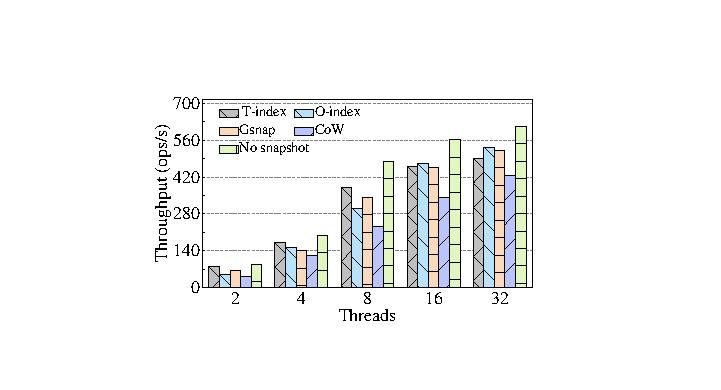
\includegraphics[width=0.8\columnwidth]{figures/ceph_pic/eval_overview.pdf}
	\caption{Throughput }
	\label{fig:databasethroughput}
\end{figure}

As shown in Figure \ref{fig:databasethroughput}, GSnap outperforms the O-index for database workloads. The reason is that GSnap reduces the number of nodes, when the file system writes a new data block, Gsnap could directly look up the index to locate the target data block, while O-index needs to generate a node and then process it.
But as the number of threads increases, the times of writing data blocks increases, and the nodes of the tree tend to be saturated, so O-index and GSnap are basically the same in index locating cost, so the number of transactions they process is also close. GSnap is lower than No-snapshot by 9\%. The reason is that the copy operation of the data block is reduced in RoW, but the snapshot still copies the uncovered data to the current object. The transaction throughput is affected by the database workload. We discuss the read/write ratio on snapshot performance in Section \ref{IPerforamce}.

\subsection{Snapshot Group Length}
In this subsection we discuss the impact of snapshot group length on snapshot recovery. Since the snapshot update ratio and the average snapshot access length determine the length of the latter group, we fix the parameters and only measure the impact of the snapshot length on snapshot recovery. We create 100 snapshots to evaluate snapshot recovery and then randomly recovered a snapshot group. The benefits of GSnap compared to other indexes are highlighted by statistical recovery latency and memory overhead.


\begin{figure}[htbp]
	\centering
	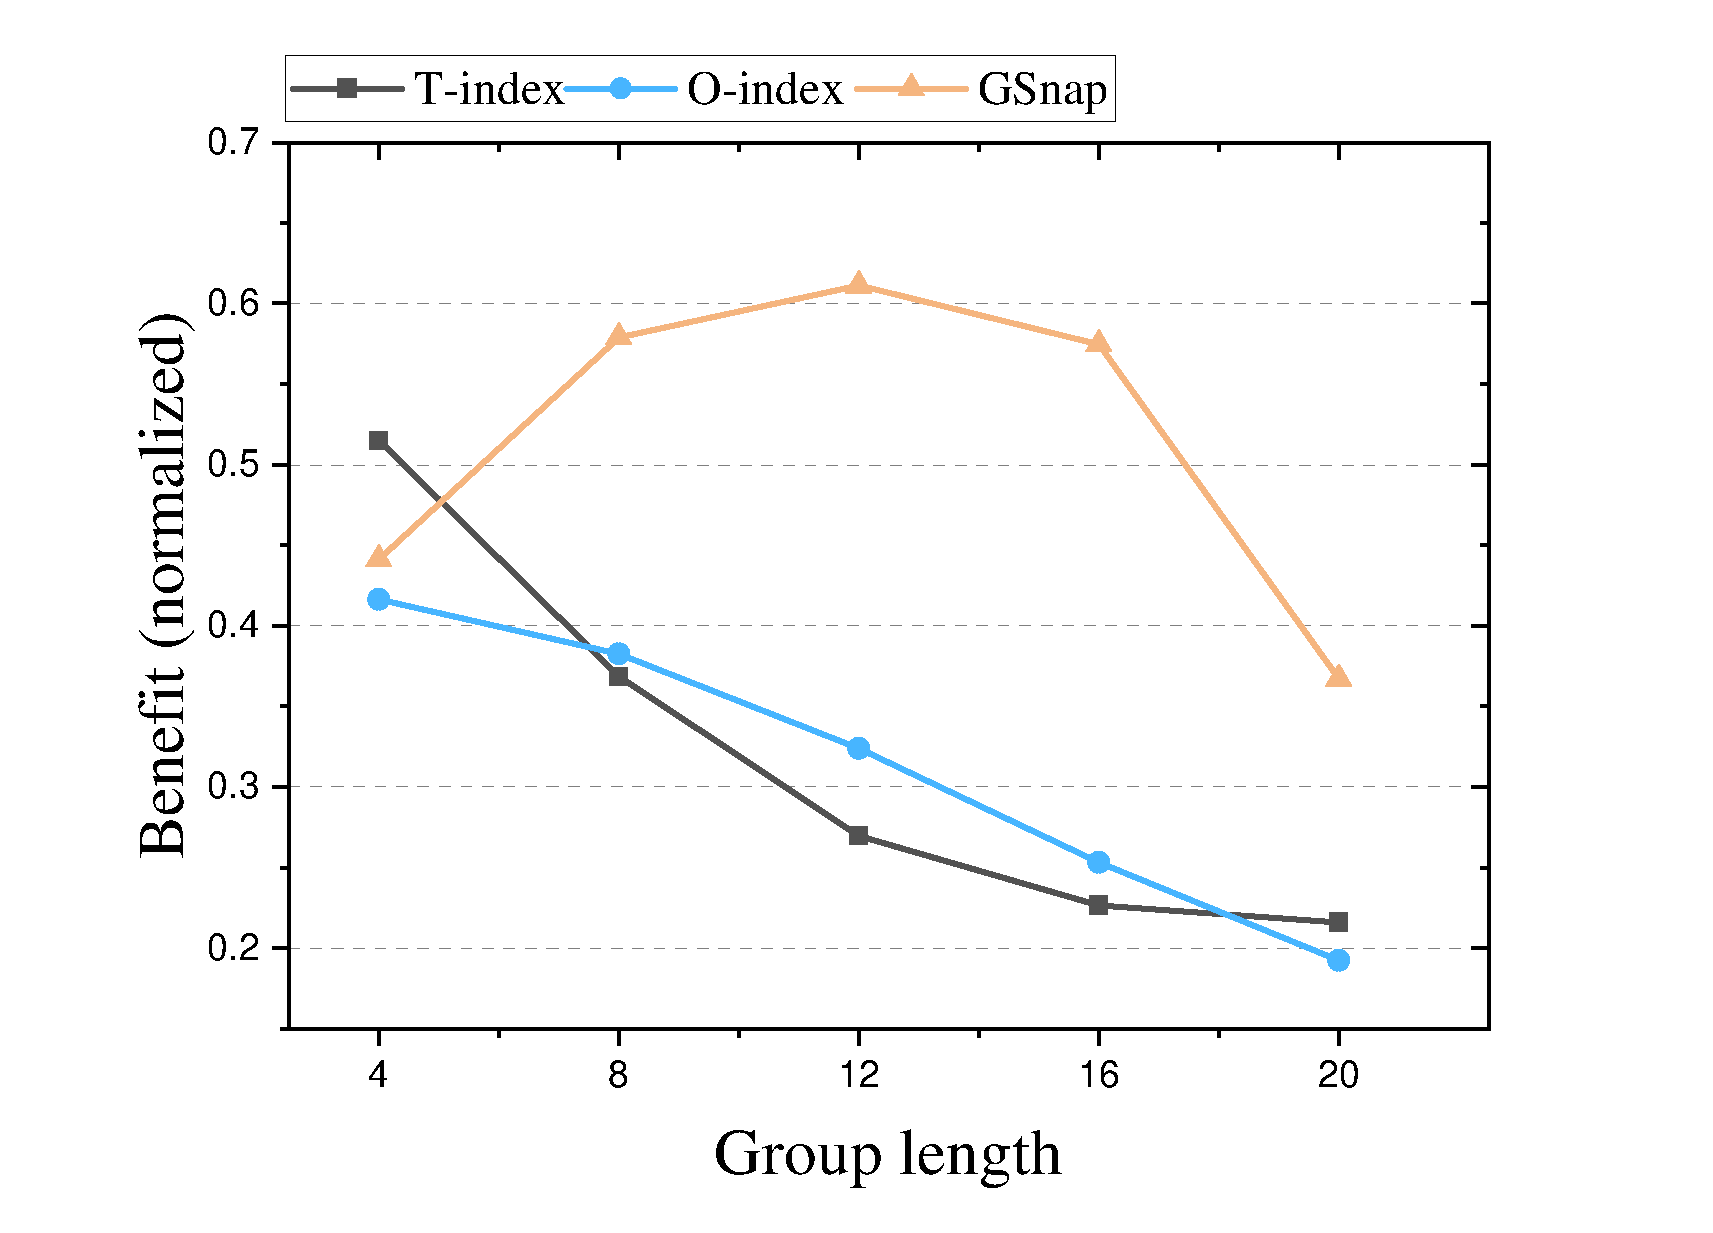
\includegraphics[width=0.8\columnwidth]{figures/ceph_pic/eval_grouplength.pdf}
	\caption{The benefit to restore a single snapshot group}
	\label{fig:grouplength}
\end{figure}


As shown in Figure \ref{fig:grouplength}, GSnap cuts off snapshot references and shares child nodes within the group, which makes its revenue higher than both T-index and O-index. Because of the snapshot dependency, T-index loads its dependent snapshot indexes when restoring the snapshot collection, and in fact, the memory usage of the group is related to the length of the dependency chain. The performance of O-index degrades as the length of the snapshot set increases, because each index is a complete snapshot tree. GSnap has the largest profit when the snapshot group length is 12, which is close to the optimal value in the theoretical analysis. As the snapshot length increases, the number of snapshots that need to be loaded and the index memory increase, resulting in lower benefits, but higher than other indexes.

\subsection{Snapshot Recovery}
Before evaluating snapshot recovery, we clone all snapshots because snapshots are read-only and flush the group index out the shared memory on the client node, which ensures that the group index is loaded from the storage cluster when restoring the snapshot. The snapshots are not deleted when restoring process. There are two types of application scenarios for accessing snapshots: single snapshot and snapshot set.
Therefore, we separately evaluate the recovery performance of those indexes in the two scenarios.
We fix the length of snapshot group to 20 since the length of the snapshot group affect the snapshot recovery.

\begin{figure}[htbp]
	\centering
	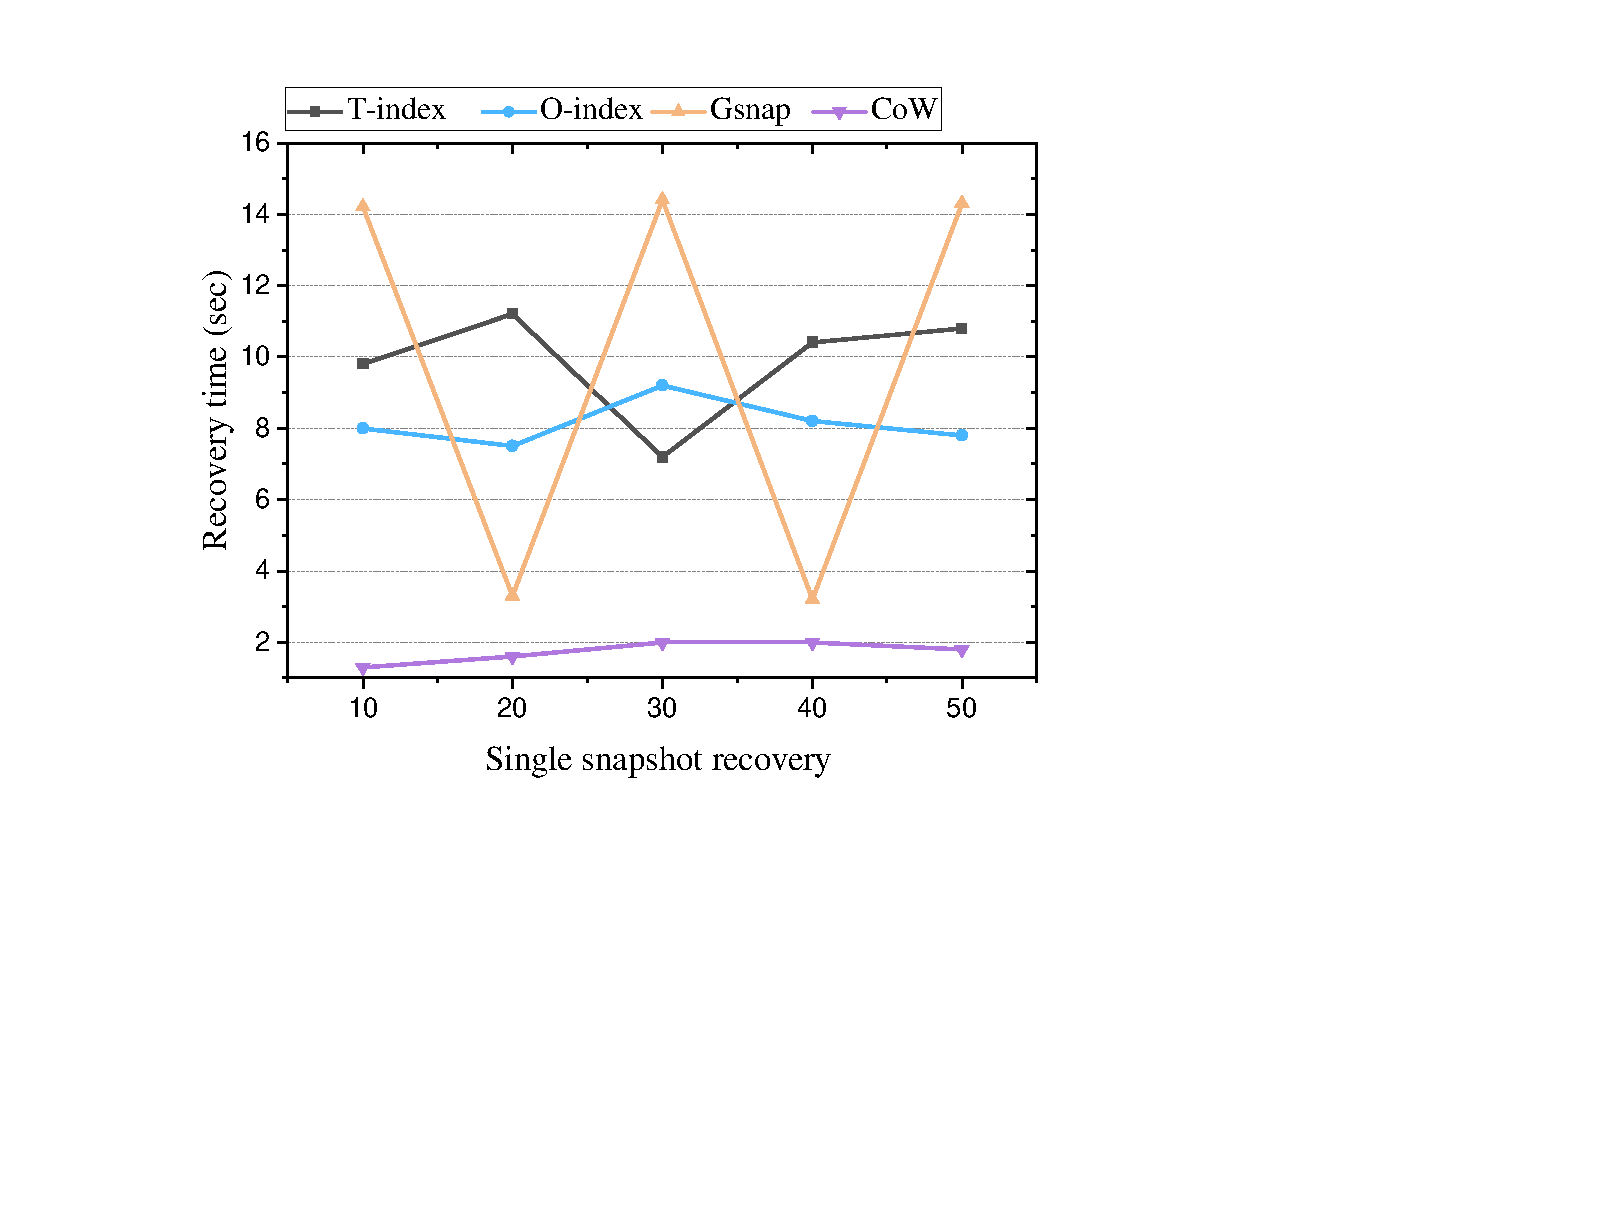
\includegraphics[width=0.8\columnwidth]{figures/ceph_pic/eval_point.pdf}
	\caption{The latency to restore a single snapshot}
	\label{fig:snapshotpoint}
\end{figure}
The recovery snapshot interval is set to 10, the purpose is to prevent the recovery of a single snapshot from evolving into the recovery of a snapshot collection and the snapshots are recovered in order. As shown in Figure \ref{fig:snapshotpoint}, we set up to restore the snapshots sequentially, so the snapshot indexes that the latter restored snapshots depend on have been loaded into shared memory.  
For GSnap, if the snapshot to be restored is already in the loaded group, the recovery latency is low, such as restoring the snapshots 20 and 40.
But the recovery delay of GSnap exceeds O-index, the reason is that GSnap needs to load more indexes than O-index.
All indexes in the group are loaded when GSnap restores a single snapshot, while O-index only needs to restore one snapshot index.

\begin{figure}[htbp]
	\centering
	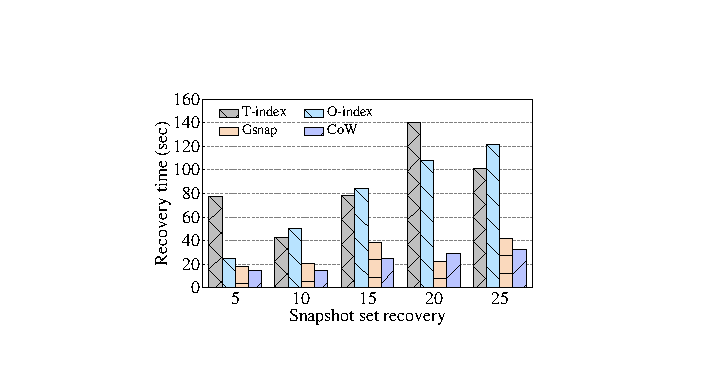
\includegraphics[width=0.8\columnwidth]{figures/ceph_pic/eval_sequence.pdf}
	\caption{The throughput to restore snapshot set}
	\label{fig:snapshotlength}
\end{figure}

We evaluate the delay of restoring snapshot sets of different lengths, to simulate continuous access to snapshots. We set all snapshot sets to randomly restore from the groups, and refresh the shared memory after each recovery operation to ensure the latency accuracy.
As shown in Figure \ref{fig:snapshotlength}, compared with O-index, the speedup of GSnap is up to 79\%, because in the loaded snapshot indexes, only 2 indexes are complete snapshot trees, and the others are partial snapshot trees, which can effectively reduce the index size of the transfer process. 
The recovery time of T-index deteriorates when restoring 20 snapshots, the reason is that the serial number of the first snapshot in recovery set is 34 and the dependency length of T-index is long.


\subsection{Snapshot Deleting}
In order to keep the number of snapshots constant, the system continuously deletes snapshots sparsely. We evaluate the latency of deleting snapshot sets of different lengths to keep the important snapshots. Besides, we also measure the overhead of merging the groups.
Since CoW does not depend on previous snapshots, we only compare O-index, T-index and GSnap. 


\begin{figure}[htbp]
	\centering
	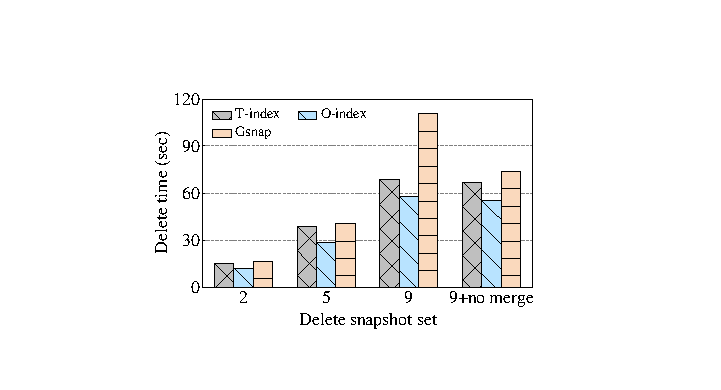
\includegraphics[width=0.8\columnwidth]{figures/ceph_pic/eval_delete.pdf}
	\caption{The latency to delete snapshot set}
	\label{fig:delete}
\end{figure}


As shown in Figure \ref{fig:delete}, when GSnap deletes snapshots, the latency is close to T-index when the snapshot length is short, only higher than 8\%. This is because when GSnap deletes an index, it needs to traverse all leaf nodes to determine whether the data block can be deleted. We add an additional set of snapshot delete operation for the unmerged group, and merge operations degraded performance by only 26\%. The reason is that 11 partial trees are left in the second group that triggered the merge operation, which increases the traversal overhead. The time of snapshot deletion is longer than GSnap due to the data merge and the index deletions operations. 
However, this cost makes the largest benefits to the performance of critical snapshot operations. 
First, the efficient snapshot creation operations make a small impact on its applications, thereby maintaining business continuity in a cloud computing environment. Second, the frequency of snapshot creation is much higher than the frequency of snapshot deletion.

\subsection{Object Size}
In this subsection, we evaluate the impact of different object sizes on index overhead and counter the proportion of the actual write size in the data block. 
Under the RoW mechanism, if the object is not fully written, the uncovered data needs to be copied from the previous snapshot to the current snapshot state. We set a balanced read-write ratio because this value affects the saturation of the snapshot index. 
We create 10 groups and randomly load snapshot groups, T-index and O-index load the corresponding snapshot sets. Finally we evaluate the memory consumption of the indexes.

\begin{figure}[htbp]
	\centering
	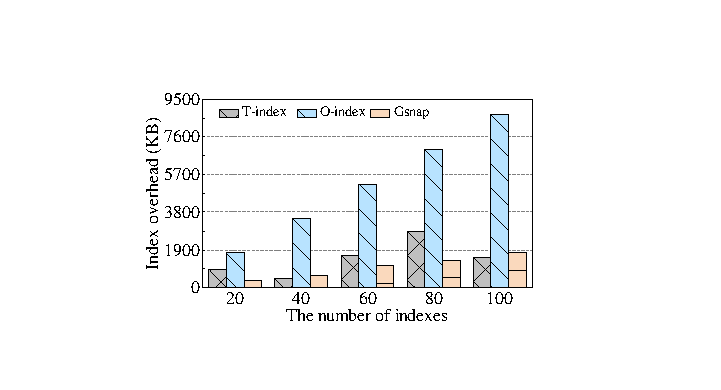
\includegraphics[width=0.8\columnwidth]{figures/ceph_pic/eval_indexmemory.pdf}
	\caption{The index overhead of snapshot}
	\label{fig:objectsize}
\end{figure}
\vspace{-0.3cm}

As shown in Figure \ref{fig:objectsize}, the index overhead of O-index exceeds that of GSnap, even though the number of the object decreases as the size increases. The reason is that O-index is the complete snapshot tree, whereas in Gsnap, only the first index within the group is a complete snapshot tree, and the remaining indexes are partial snapshot trees. the design of the group dilutes the average number of nodes. The index overhead of GSnap is only 8\% higher than that of T-index because the average indexing overhead is diluted by other partial indexes within the group.
As the object size increases, the actual data write ratio decreases. The reason is that at the end of the snapshot, the system checks the coverage area of all objects and copies the default content from the previous objects to the current object.

\subsection{Merge Length}
In this subsection, we evaluate the effect of numbers of indexes in the latter group in the merge operation. Likewise, we set the length of the snapshot group to 20, and the recovered snapshot collection to 10. We randomly restore the set of snapshots to avoid trapping in a single group.

As shown in Figure \ref{fig:merge}, the merge overhead increases with the number of partial snapshots in the second group, because each index needs to be traversed and merged into the previous group.
We evaluate load delay reduction of 28.7 seconds for one group, which is the benefit time of merging group. This delay is higher than the merge overhead when the number of the partial tree is 5 in the latter group, which means that the merge is only profitable at this time. The snapshot group length is related to the average access length, so the number of partial snapshots in the second group also dynamically adapts to user access behavior when merging groups. As shown in Figure \ref{fig:merge_recovery}, the more partial snapshots left when the merge operation is initiated in the second group, the lower the recovery latency. The reason is that most of the groups have been merged and the snapshots within the group are saturated, so only one group is restored. When there are 1 or 5 partial indexes in the group, merge operations are reduced. Thus the collection needs to restore two groups leading to increasing recovery overhead.

%\vspace{-0.3cm}
%\begin{figure}[htbp]
%	\centering
%	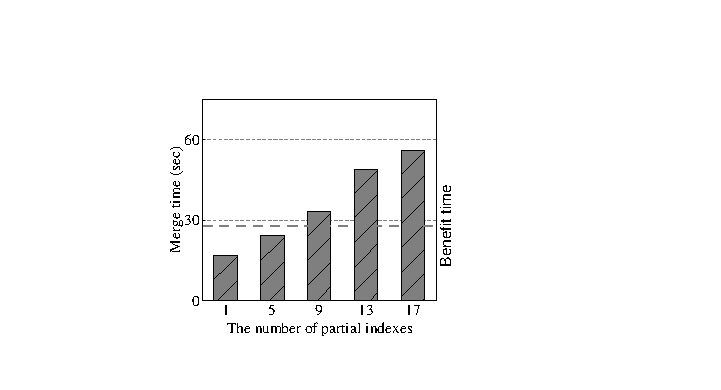
\includegraphics[width=0.8\columnwidth]{figures/ceph_pic/eval_merge.pdf}
%	\caption{The latency to delete snapshot set}
%	\label{fig:merge}
%\end{figure}
%\vspace{-0.3cm}
%
%\vspace{-0.3cm}
%\begin{figure}[htbp]
%	\centering
%	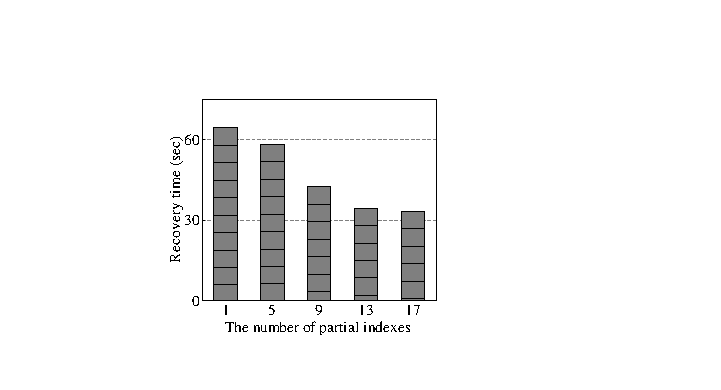
\includegraphics[width=0.8\columnwidth]{figures/ceph_pic/eval_merge_recovery.pdf}
%	\caption{The latency to delete snapshot set}
%	\label{fig:merge_rec}
%\end{figure}
%\vspace{-0.3cm}


%\begin{figure}[htbp]
%	\centering
%	\subfigure[Write-Only]{
%		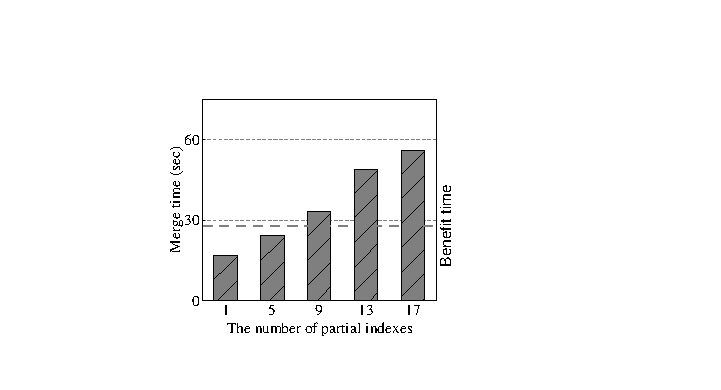
\includegraphics[width=0.5\columnwidth]{figures/ceph_pic/eval_merge.pdf}
%		\label{read-only}}
%	\subfigure[Balanced]{
%		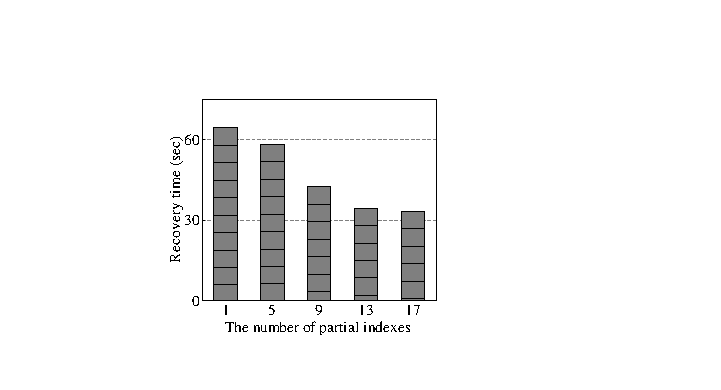
\includegraphics[width=0.5\columnwidth]{figures/ceph_pic/eval_merge_recovery.pdf}
%		\label{banlanced}}
%	\caption{The I/O performance for GSnap}
%	\label{fig:IO_performance}
%\end{figure}
\vspace{-0.3cm}
\begin{figure}[htbp]
	\begin{minipage}[t]{0.45\linewidth}
		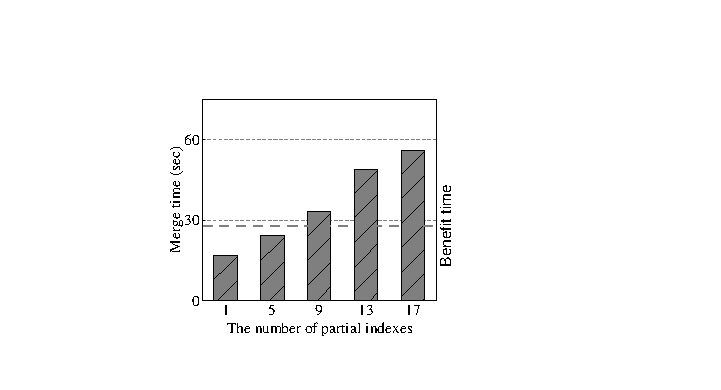
\includegraphics[width=\linewidth]{figures/ceph_pic/eval_merge.pdf} 
		\caption{The latency of recovering snapshot set} 
		\label{fig:merge}
	\end{minipage}%
	\hfill%
	\begin{minipage}[t]{0.45\linewidth}
		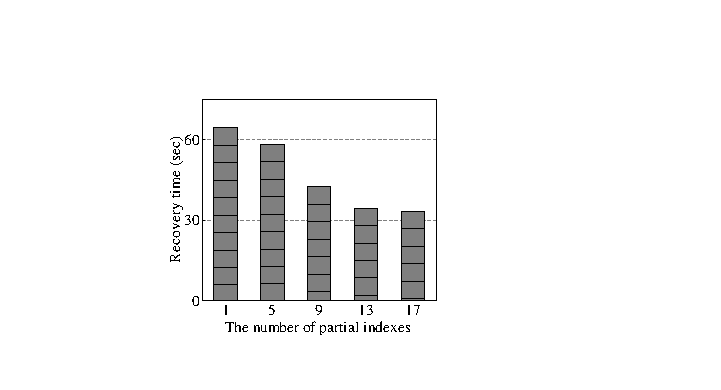
\includegraphics[width=\linewidth]{figures/ceph_pic/eval_merge_recovery.pdf}
		\caption{The latency of merging groups}
		\label{fig:merge_recovery}
	\end{minipage} 
\end{figure}
\vspace{-0.3cm}

\subsection{I/O Performance}


\begin{figure*}[htbp]
	\centering
	\subfigure[Write-Only]{
		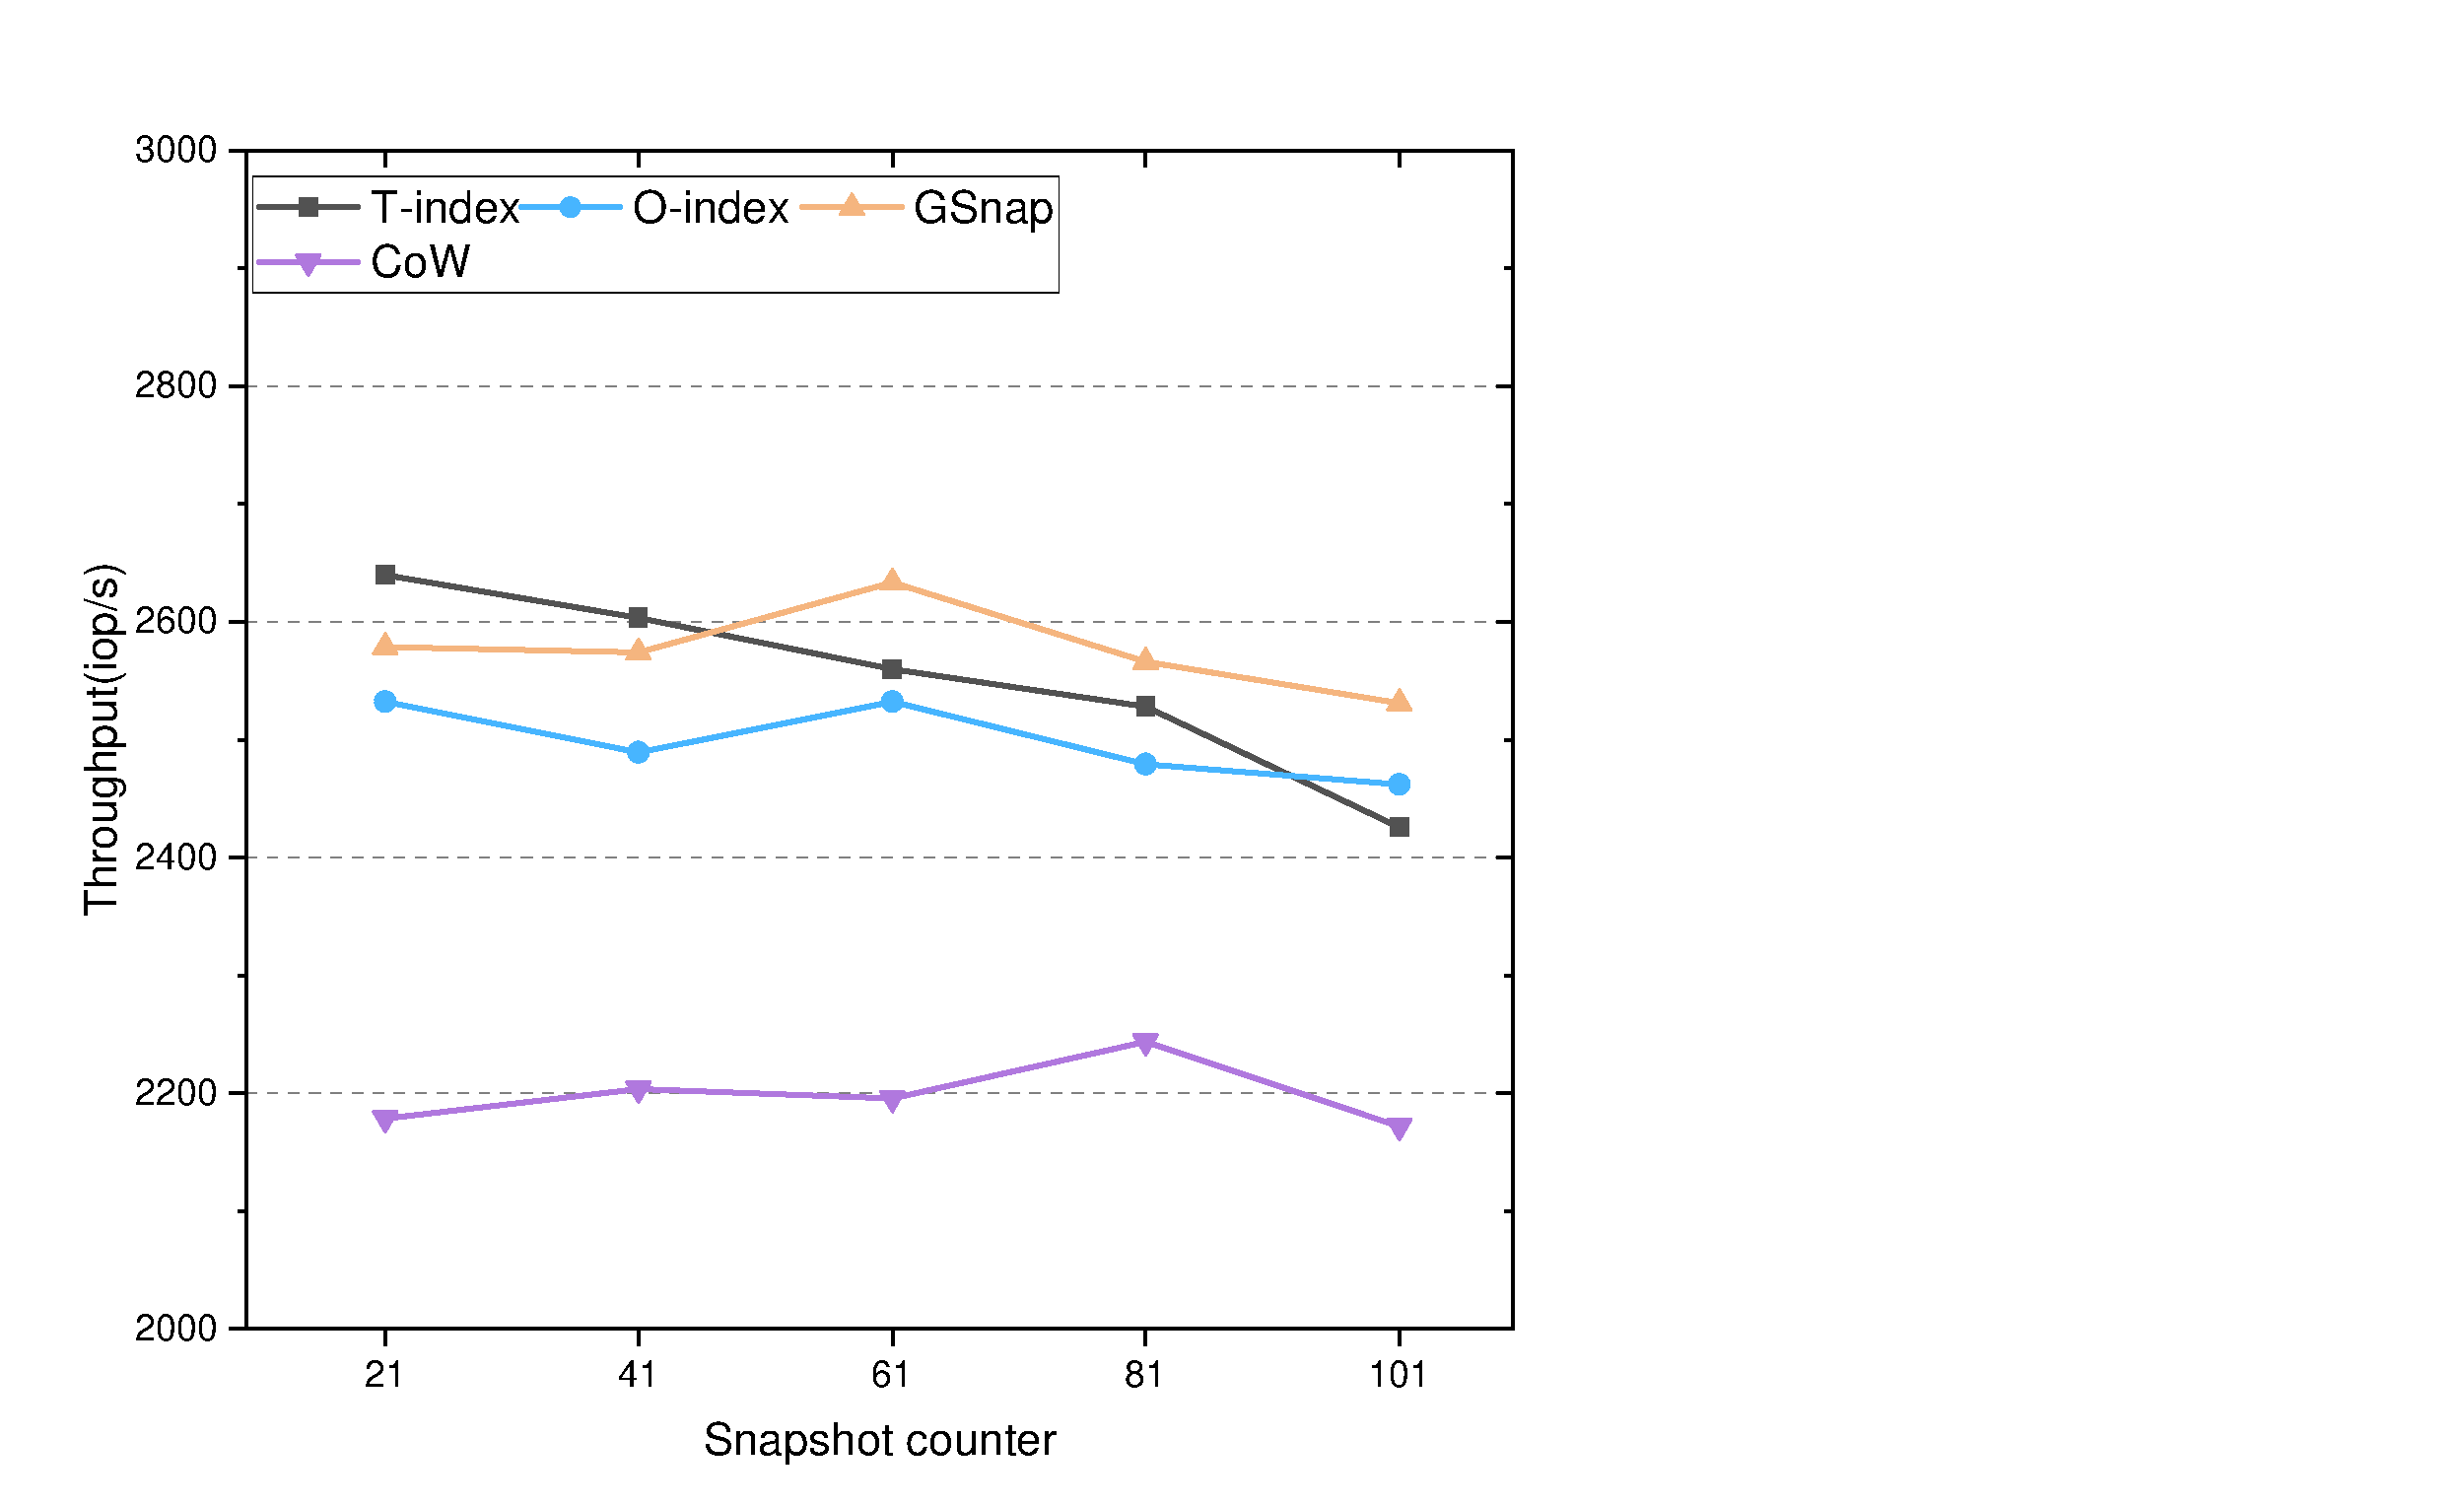
\includegraphics[width=6cm]{figures/ceph_pic/eval_write.pdf}
		\label{read-only}}
	\hspace{-5in}
	\subfigure[Balanced]{
		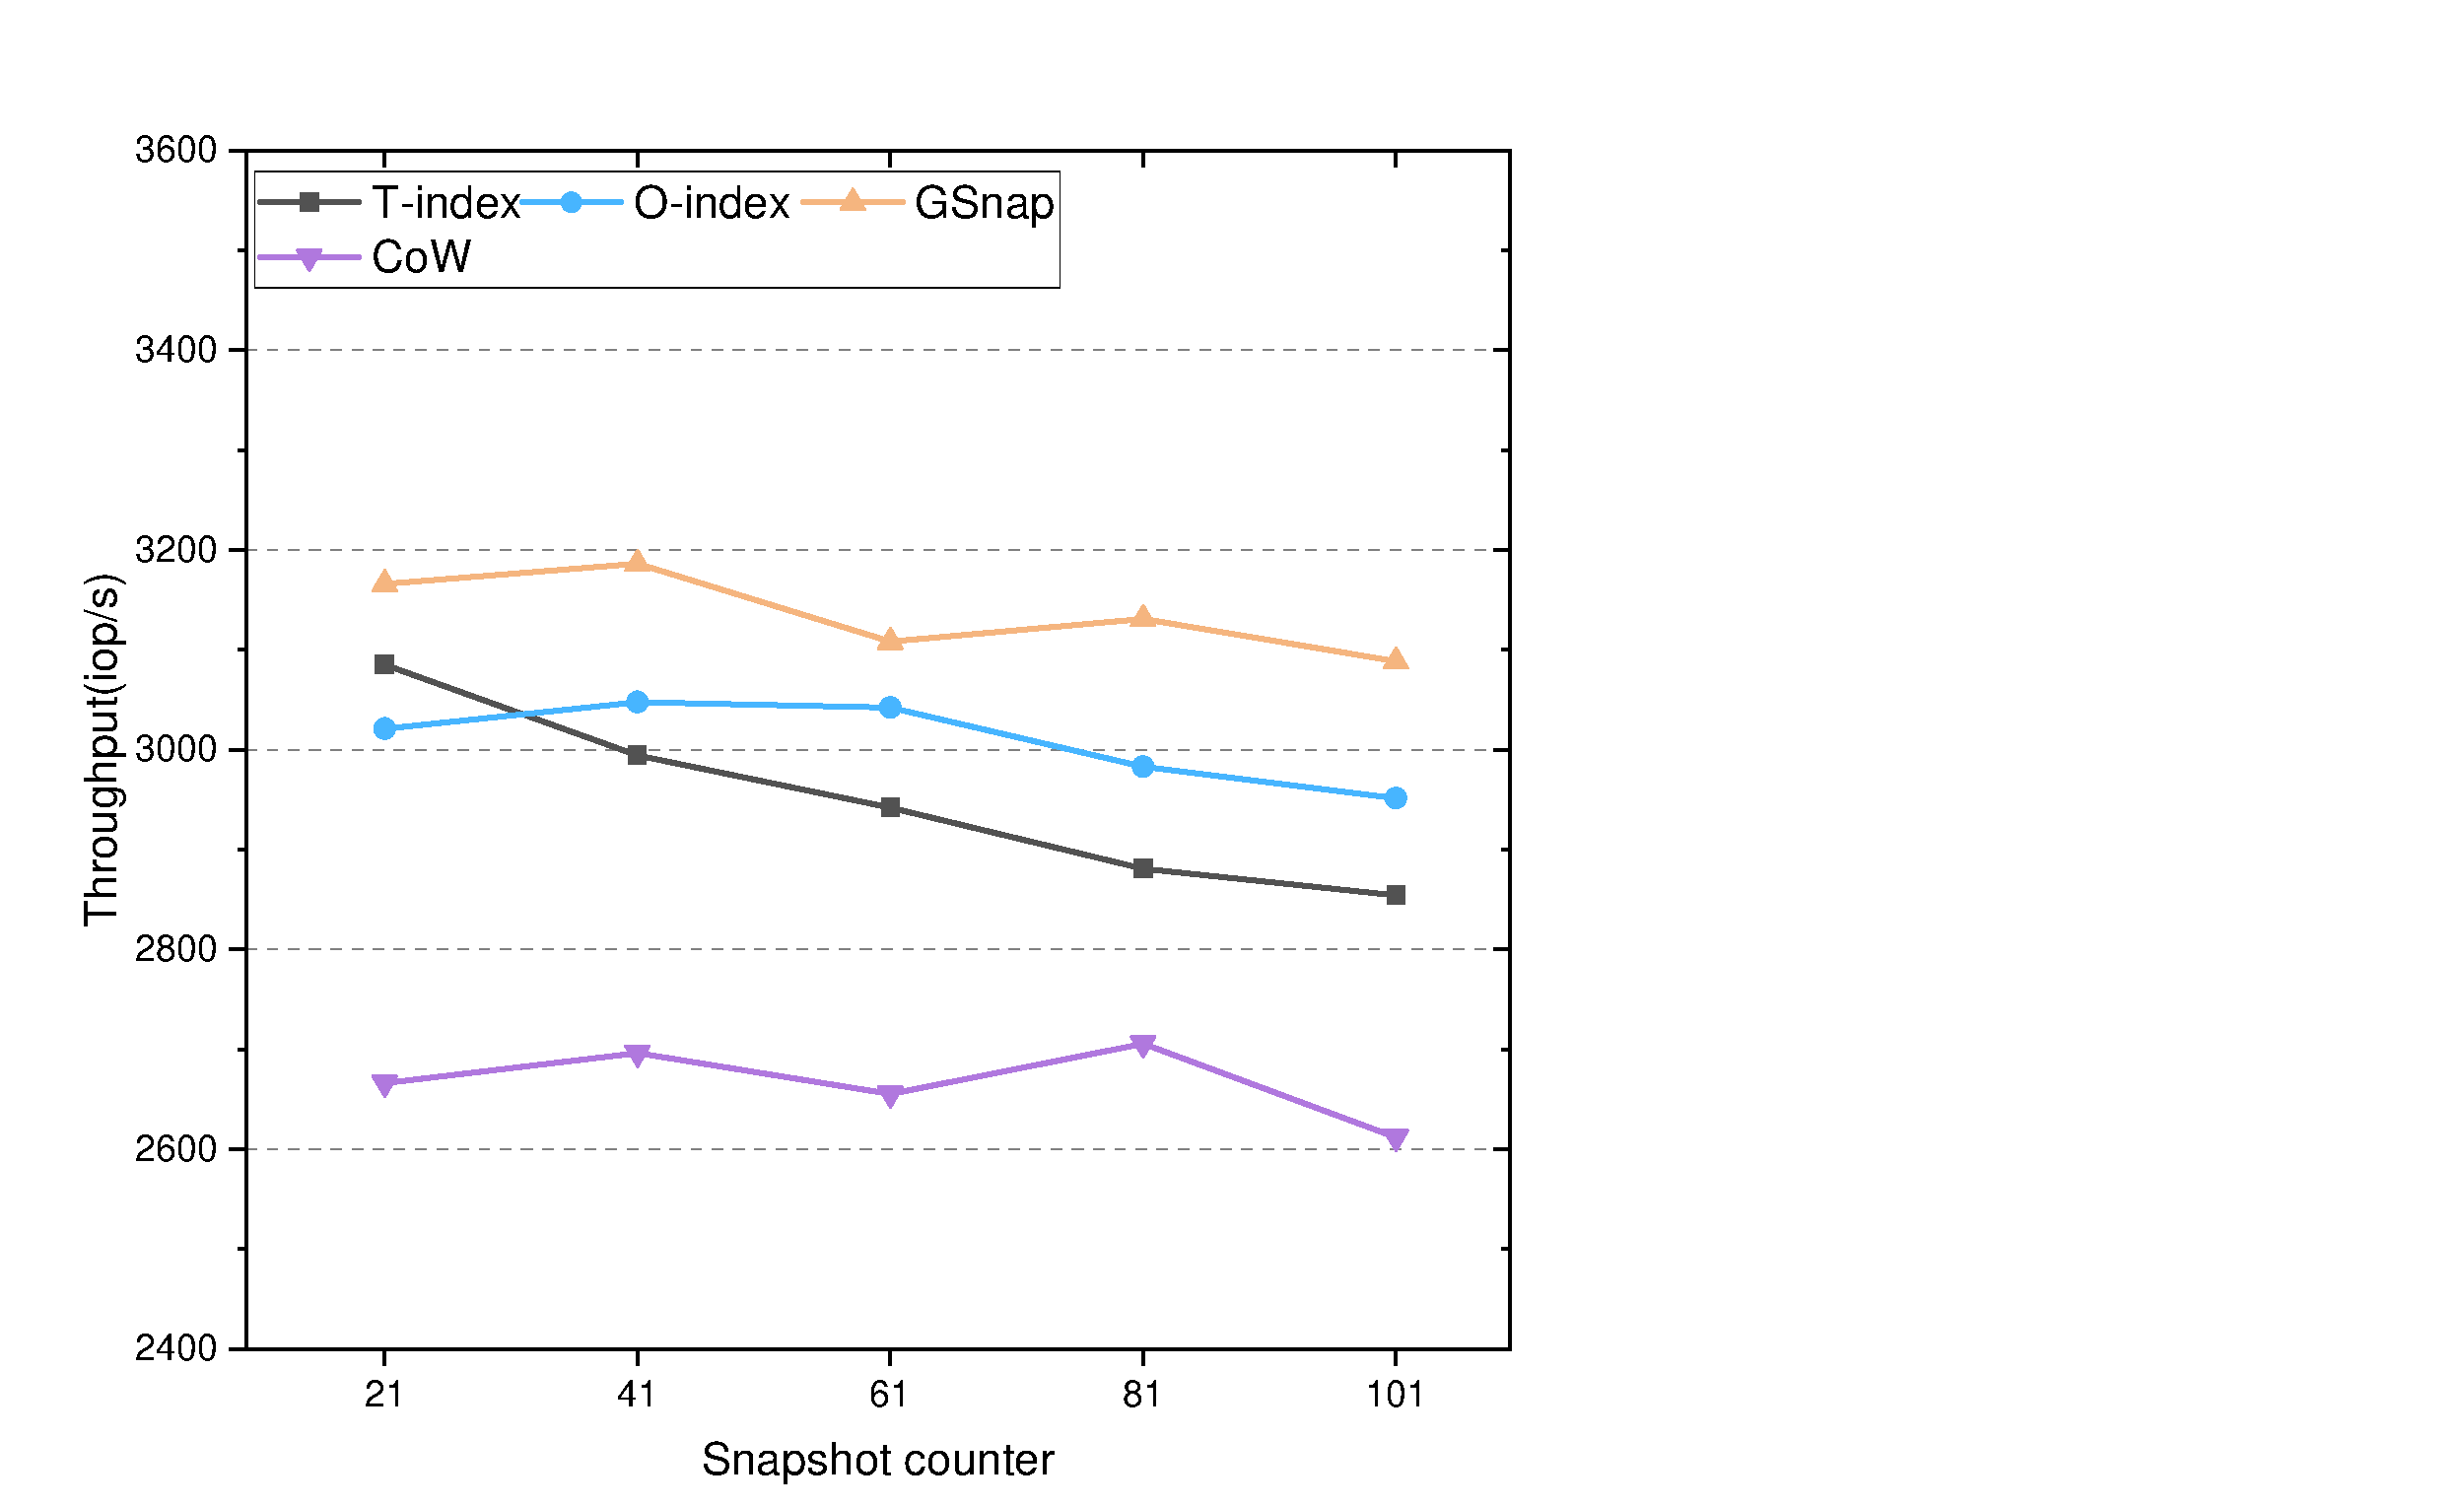
\includegraphics[width=6cm]{figures/ceph_pic/eval_balanced.pdf}
		\label{banlanced}}
	\hspace{-5in}
	\subfigure[Read-Only]{
		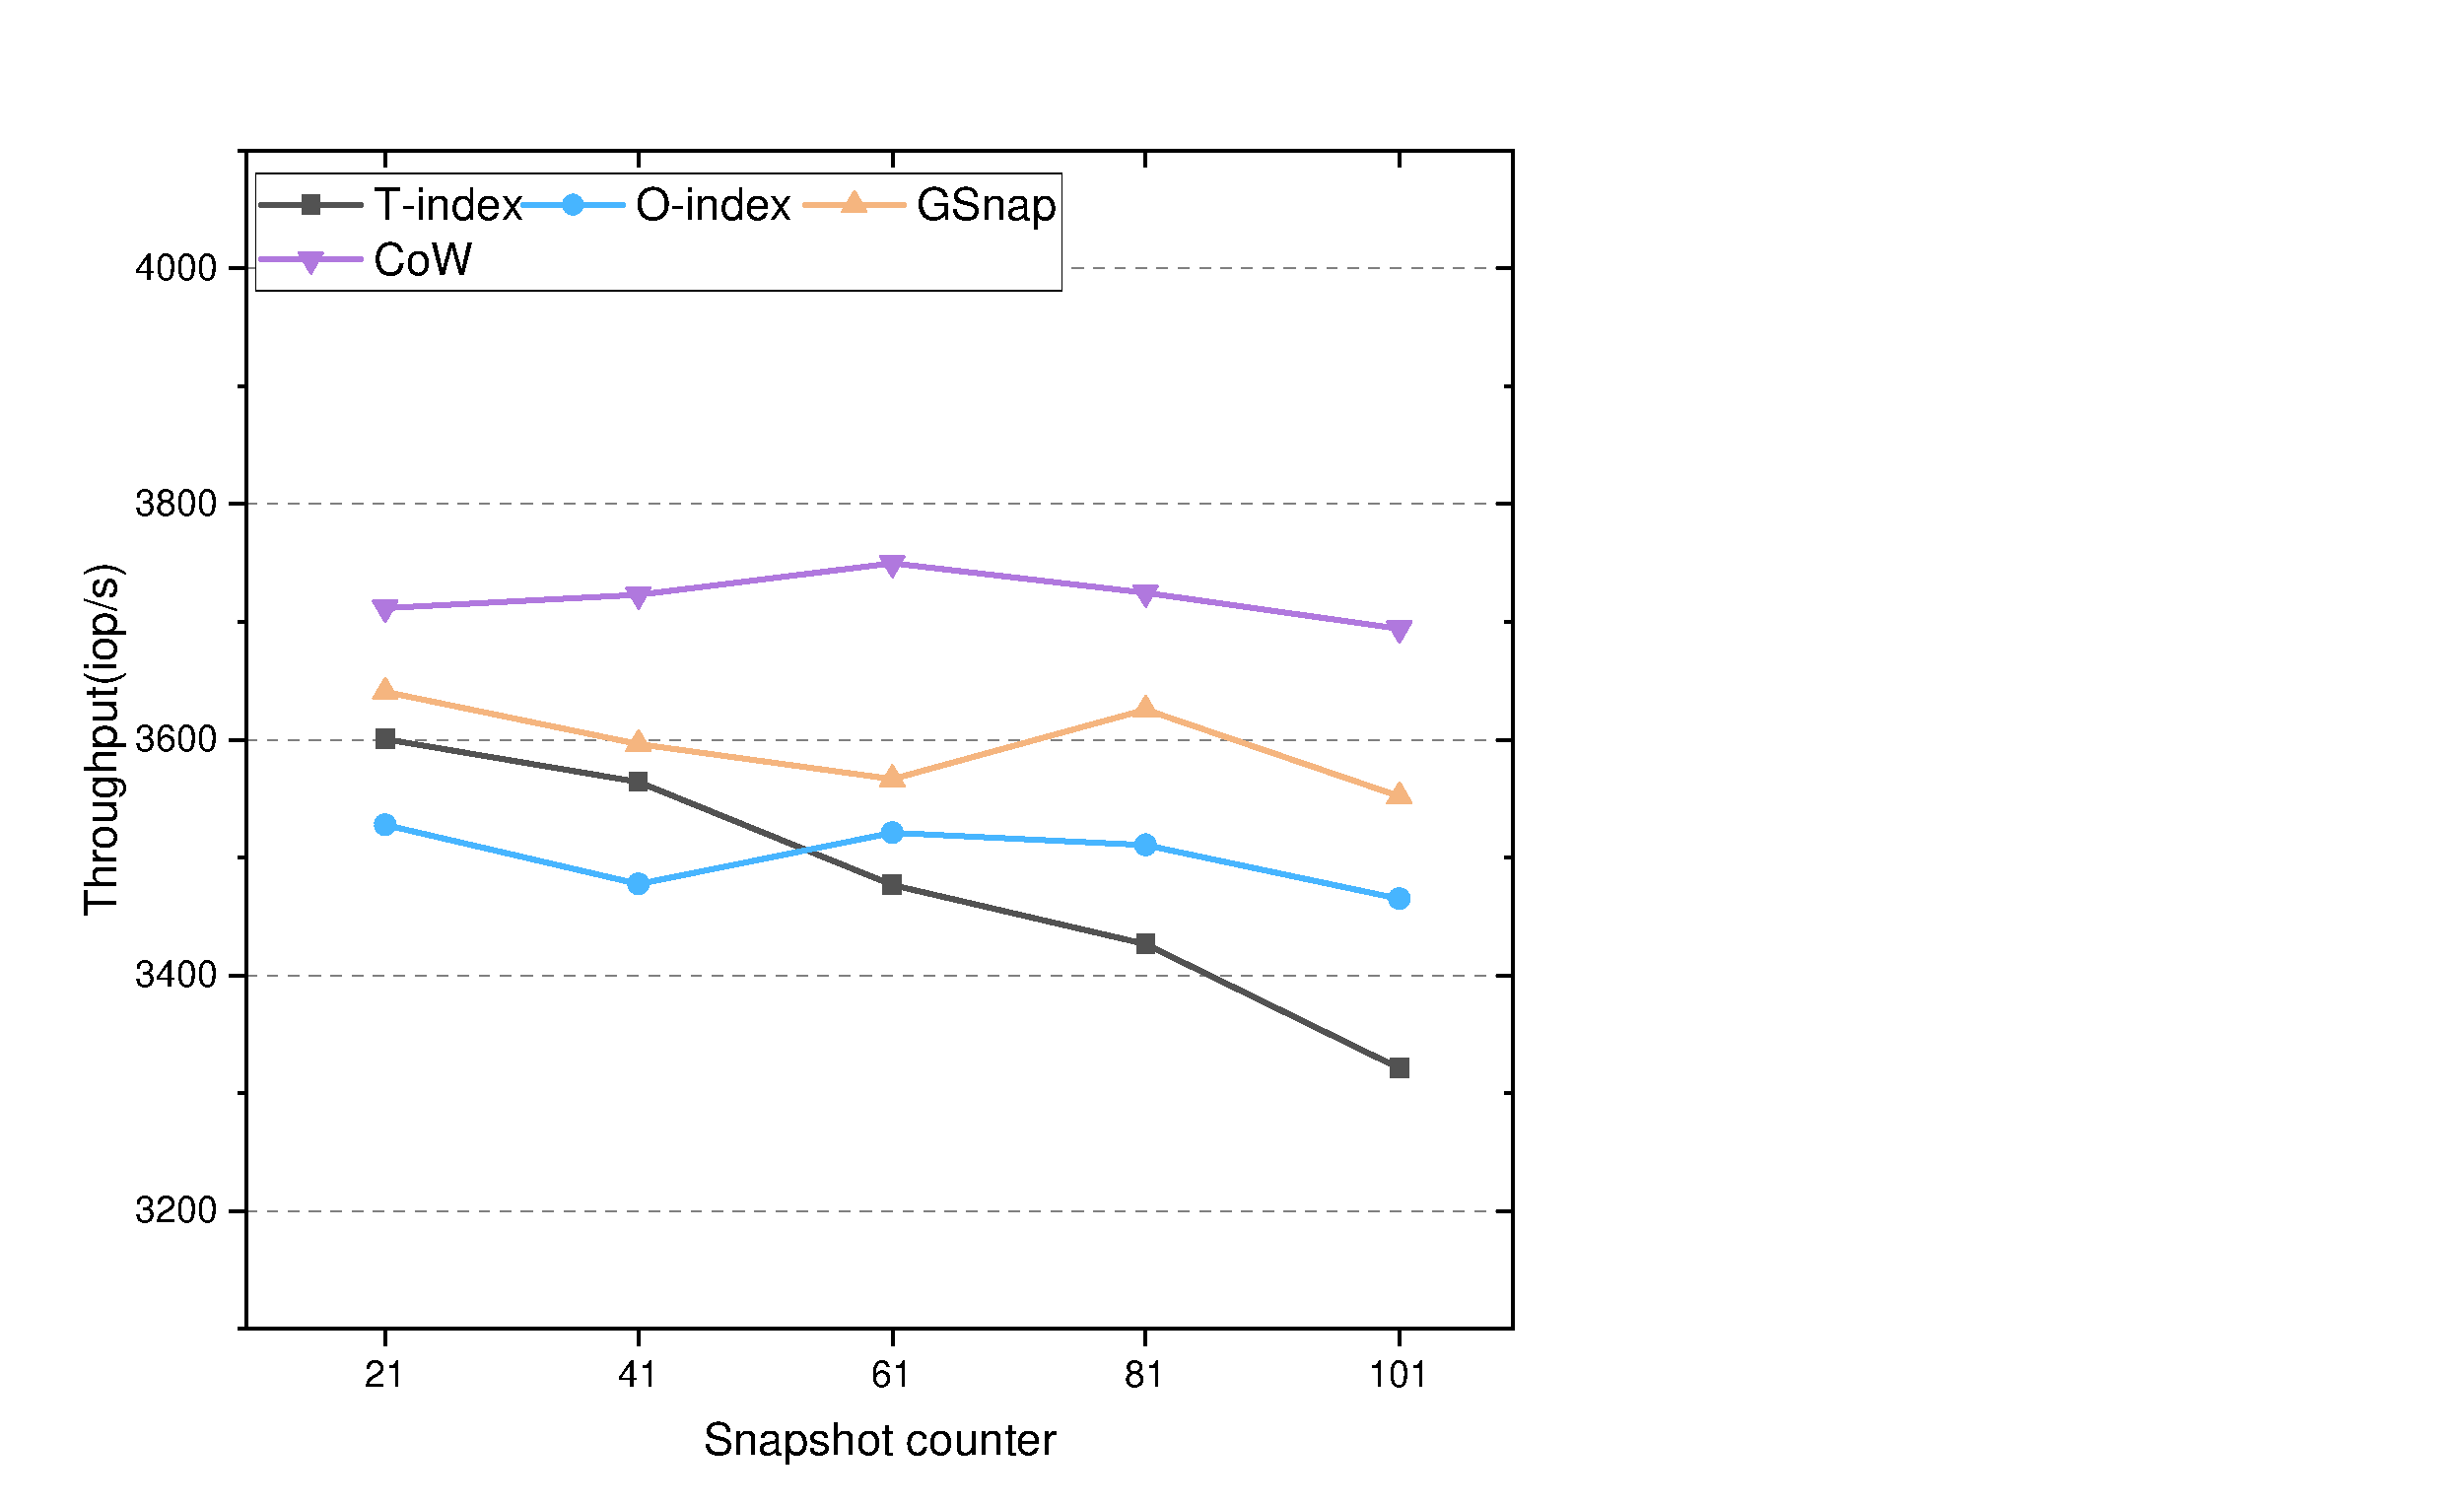
\includegraphics[width=6cm]{figures/ceph_pic/eval_read.pdf}
		\label{write-only}}
	\caption{The I/O performance for GSnap}
	\label{fig:IO_performance}
\end{figure*}

\label{IPerforamce}
We also evaluate the I/O performance in the XFS and compare the throughput under various number of snapshot, highlighting the impact of indexes on locating data blocks. Specifically, the read/write ratio set as: read-only, balanced (50\% read / 50\% write) and write-only. the block size is default set to 4MB.

As shown in Figure \ref{fig:IO_performance}, the performance of gsnap is stable as the number of snapshots increases. The reason is that the group cuts off the dependency of snapshots. When locating data blocks, only the snapshots in the group need to be accessed. Even if O-index only needs to access the previous snapshot, it copies all leaf nodes. Of course, the performance of the first snapshot in the group is lower than O-index since it accesses the prior group and constructs a complete index. In read-only workloads, CoW performs better than other indexes because only the current snapshot needs to be accessed. As the write ratio increases, the performance degrades significantly due to the double write.
The performance of T-index decreases as the number of snapshots increases in read-only workloads. Because it needs to access indexes iteratively when looking for data blocks. As shown in Figure \ref{write-only}, the iterative traversal of data blocks is reduced in the write-only workload, the performance is still degraded. The reason is that the lazy eviction of the previous indexes leads cache overhead increase.

\section{Related work}
\label{Relatedwork}
\textbf{Snapshot Technologies.}
Snapshot Implementations such as: CoW, CoW with background copy (CoW+), Split Mirror Redundant Array of Independent Disks (SMRAID), Incremental Snapshot, Continuous Data Protection (CDP) \cite{garimella2006understanding}, RoW. The snapshot technologies have been extensively compared and analysed \cite{mahipal2021virtual,joseph2019securing,almulla2013distributed,subramanian2014snapshots}. CDP is made incrementally and used  in synchronous data mirroring  and Incremental Snapshot adapts a timestamp-based incremental approach with rollback provisioning. In summary, the write overhead of CoW, CoW+, SMRAID are suffered by their methodologies, their derivative technologies induce overheads for regular I/O and dramatic increase of sync operations when snapshots are present \cite{subramanian2014snapshots,li2012irow}. 
%Incremental Snapshot and CDP are mostly dependent on the underlying technology used for taking snapshots and network bandwidth.
Traversing to locate data blocks can cause performance degradation because fragmentation increases as snapshots increase.
Amazon EBS \cite{varia2014overview} has an optimized RoW snapshot index that stores the regions which are continuous unchanged data blocks. The region points to the last changed snapshot instead of the previous snapshot to avoid iterative queries.
However, when the number of snapshots grows, the size of each region shrinks and the number of regions grows, considerably increasing the memory footprint of indexes.

\textbf{Index Structure.}
\cite{DBLP:conf/icpads/LiZCY14} uses the bitmap method to record the block number, but in the RoW, the dependency relationship still exists between the snapshots, and there is an iterative traversal to find the data block. \cite{tsikoudis2018rql,shrira2005snap,tsikoudis2020rid} use a log structure to record snapshot metadata, and the metadata updating overhead of log structure is heavy when snapshots are continuously added and deleted. Parallax \cite{DBLP:conf/eurosys/MeyerACLFHW08} leverages a tree structure to maintain snapshot indexes, and adopt ratix tree to reduce leaf nodes overhead. We also adopt the ratix tree structure and borrow the ZFS \cite{rodeh2003zfs} to share child nodes between trees to reduce indexing overhead. Amazon EBS \cite{varia2014overview} optimizes the structure of the leaf node on the optimized index, setting fixed-length leaf nodes to store continuous unmodified data blocks to reduce the memory consumption of the index. However, the leaf node locating becomes complicated and the overhead of index updating increases when the snapshot is updated. Moreover, as the write ratio increases, the index degenerates the optimized index. Therefore, it is not applicable for the scenario of accessing a large number of snapshots.

\textbf{Snapshot Implementation Layers.}
In the database layer, database administrators can choose mysqldump \cite{mysqldump} for logical backup and Percona Xtrabackup \cite{xtrabackup} for physical backup. A logical backup stores the queries executed by transactions, while the physical backup copies the raw data to storage. In the recovery process, the stored queries are re-executed, or backup data are copied to a database directory. However, recovery operations in the existing tools take a long time, since these recovery procedures involve a large amount of I/O operations induced by database queries or raw data copies.
Snapshots techniques supported by file systems and the block layer can be adopted for the backup and recovery of database. Network Appliance NAS filers, the Sun ZFS \cite{rodeh2003zfs} and BTRFS \cite{rodeh2013btrfs} organize the file as a tree with data at the leaf level and meta-data maintained in internal nodes.
%Each snapshot consists of a separate tree, but snapshot may share subtrees with other snapshots.  
%Though creating a snapshot is lightweight, the overhead of first write to a block is heavy once a snapshot is created because the entire tree of meta-data nodes needs to be copied and linked to the root node of the snapshot. 
LVM \cite{hasenstein2001logical} operates the storage device and provides fast snapshot creation and restoration using CoW. However, the CoW negatively affects run-time performance since it performs redundant writes due to data copies.

\section{conclusions}
\label{Conclusions}
In this paper, we propose GSnap, a lightweight RoW-based snapshot index for large-scale backup and fast recovery. It performs a hybrid design to split the dependency of snapshot indexes in a group. In-group snapshot indexes reduce memory overhead by sharing subtrees. The index can directly locate data blocks instead of iterative traversal. Loading target snapshot group indexes instead of indexes dependent, which balances index memory and recovery time overhead. 
The experimental results show that GSnap achieves higher performance than
compared indexes.

\begin{acks}
\end{acks}

%\clearpage

\bibliographystyle{ACM-Reference-Format}
\bibliography{ref}

\end{document}
\endinput
